\section{Color Chaos}

Chen claimed in \cite{pchen}, that correlation analysis and spectral analysis are complementary tools in the stationary time-series analysis. Based on the detail study of the paper \cite{pchen}, \textbf{Color Chaos} is defined as a time frequency representation as a nonparametric approach for generalized spectral analysis for evolutionary time series. In color chaos, the HP filter is applied for trend-cycle decomposition and time-variant filters in Gabor space for pattern recognition.  Discrete-time white chaos generalized by nonlinear difference equations is tractable analytically and from the needs of empirical analysis, the continuous-time color chaos generated by nonlinear differential equations is more capable of describing business cycles than white chaos, since fluctuations and recurrent patterns can be characterized by nonlinear oscillations with irregular amplitude and a narrow frequency band in the spectrum.  Chen claimed in \cite{pchen}, the newly decoded deterministic signals from persistent business cycles reveal new sources of market uncertainty, such as changing growth-trend and shifting business cycles. 


\subsection{Role of time scale \& reference trends in representation of business cycles}

A distinctive problem in economic analysis is how to deal with growing trends in an aggregate economic time series. Both level and rate information are important when correlations are not short during business cycles. 

\textit{Time Scale}:
Chaos theory in nonlinear dynamics emphasizes the role of history, because a nonlinear deterministic system is sensitive to its initial condition. The martingale theory of the stock market ignores the path-dependent information in the stock market. The challenges faced are:
\begin{enumerate}
\item Choosing an appropriate time sampling rate is often ignored in econometric analysis. Chaotic cycles in continuous time may look like noise if the sampling time interval is not small compared to its fundamental period of a cycle.  For example, annual economic data are not capable of revealing the frequency pattern of a business cycle. 
\item Numerically, a large time unit such as the annual time series can easily obscure a cyclic pattern in the correlation analysis of business cycles.
\end{enumerate}
\textit{Reference Trend}:
How to choose a reference trend or a proper transformation to simplify the empirical pattern of business cycles? The core problem in economic analysis is not noise-smoothing but trend-defining in economic observation and decision making. There are two criteria in choosing the proper mathematical representation. 
\begin{enumerate}
\item Mathematical reliability 
\item Empirical verifiability.
\end{enumerate}
Unlike experimental economics, macroeconomic time series are not reproducible in history. Traditional tests in econometric analysis have limited power in studies of an evolutionary economy containing deterministic components.  A good fit of past data does not guarantee the ability for better future predictions.  There are two extreme approaches in econometric analysis: the trend-stationary (TS) approach of log-linear detrending (LLD) and the difference-stationary (DS) approach of first differencing (FD).  A compromise between these two extremes is the Hodrick and Prescott (HP) filter.  In principle, a choice of observation reference is associated with a theory of economic dynamics. Log-linear detrending implies a constant exponential growth as shown in the figure ~\ref{fig:LogLinear}. 

The FD detrending produces a noisy picture that is predicted by the random-walk model with a constant drift (or the so-called unit-root model in econometric literature).  Economically speaking, the FD detrending in econometrics implies that the level information in price indicators can be ignored in economic behavior.  This assertion may conflict with many economic practices, since traders constantly watch economic trends, and no one will make an investment decision based only on the current rate of price changes.  The error-correction model in econometrics tried to remedy the problem by addition some lagged-level information, such as using a one-year-before level as an approximation of the long-run equilibrium. Then comes the problem of what is the long run equilibrium in the empirical sense.  A proper decomposition of trend and cycles may find an appropriate scheme to weigh the short-term and long-run impacts of economic movements in economic dynamics.  The essence of trend-cycle decomposition is finding an appropriate time window, or equivalently, a proper frequency window, for observing time-dependent movements.  Log-linear detrending is a low-pass filter or wave detector, while first differencing is a high-pass filter or noise amplifier. 

The main drawback of LLD detrending is its over-dependence on historical boundaries, while the DS series is too erratic from amplifying high-frequency noise. 

HP filter has two advantages. 
\begin{enumerate}
\item It is localized approach in detrending, with the problem of boundary dependence. 
\item Frequency response is in the range of business cycles. 
\end{enumerate}

\subsection{Dimensionality}

\subsection{Correlation Dimension}
The correlation dimension provides a tool to quantify self-similarity. A larger correlation dimension corresponds to a larger degree of complexity and less self-similarity. The most frequently used procedure to estimate the correlation dimension was introduced by Grassberger and Procaccia (1983). They defined the correlation sum for a collection of points $X_i$ $(i=1,2,3,..,N)$ in some phase space to be the fraction of all possible pairs of points which are closer than a given distance $\epsilon$ in a particular norm:

To compute the correlation sum $C(m,\epsilon)$ and the correlation dimension $D_c$, first delay-coordinate embed the signal as follows:


$X(t) = {x(t), x(t+\tau), x(t+2\tau),..,x(t+(m-1)\tau)}$

where $\tau$ is the delay time, and $m$ is the embedding dimension. 

\begin{equation} \label{cd:1}
C(m,\epsilon) = \frac{2}{(N-m)(N-m-1)} \sum_{i=m}^{N}\sum_{j=i+1}^{N} \Theta (\epsilon - \lVert X_i - X_j \rVert )
\end{equation}

where $\Theta$ is Heaviside step function, $\Theta(x) = 0$ if $x \le 0 $ and $\Theta(x) = 1$ for $x>0$ and $X_i = X(t_i)$.
Thus equation \ref{cd:1} counts the pairs $(X_i,X_j)$ whose distance is smaller than $\epsilon$.  When ${N\to\infty}$, for small values of $\epsilon$, C follows a power law;

\begin{equation} \label{cd:2}
C(\epsilon) \propto \epsilon^{D_c}
\end{equation}

where $D_c$ is correlation dimension. Therefore, $D_c$ is defined as
\begin{equation} \label{cd:3}
D_c = \lim_{\epsilon\to 0} \lim_{N\to\infty} \frac{\partial log_{10} C(\epsilon)}{\partial log_{10}(\epsilon)}
\end{equation}

Correlation dimension is estimated by computing the slope of the straight line by using least square fit in a plot of $log_{10} C(\epsilon)$ vs $log_{10}(\epsilon)$.

\begin{figure}[!ht]
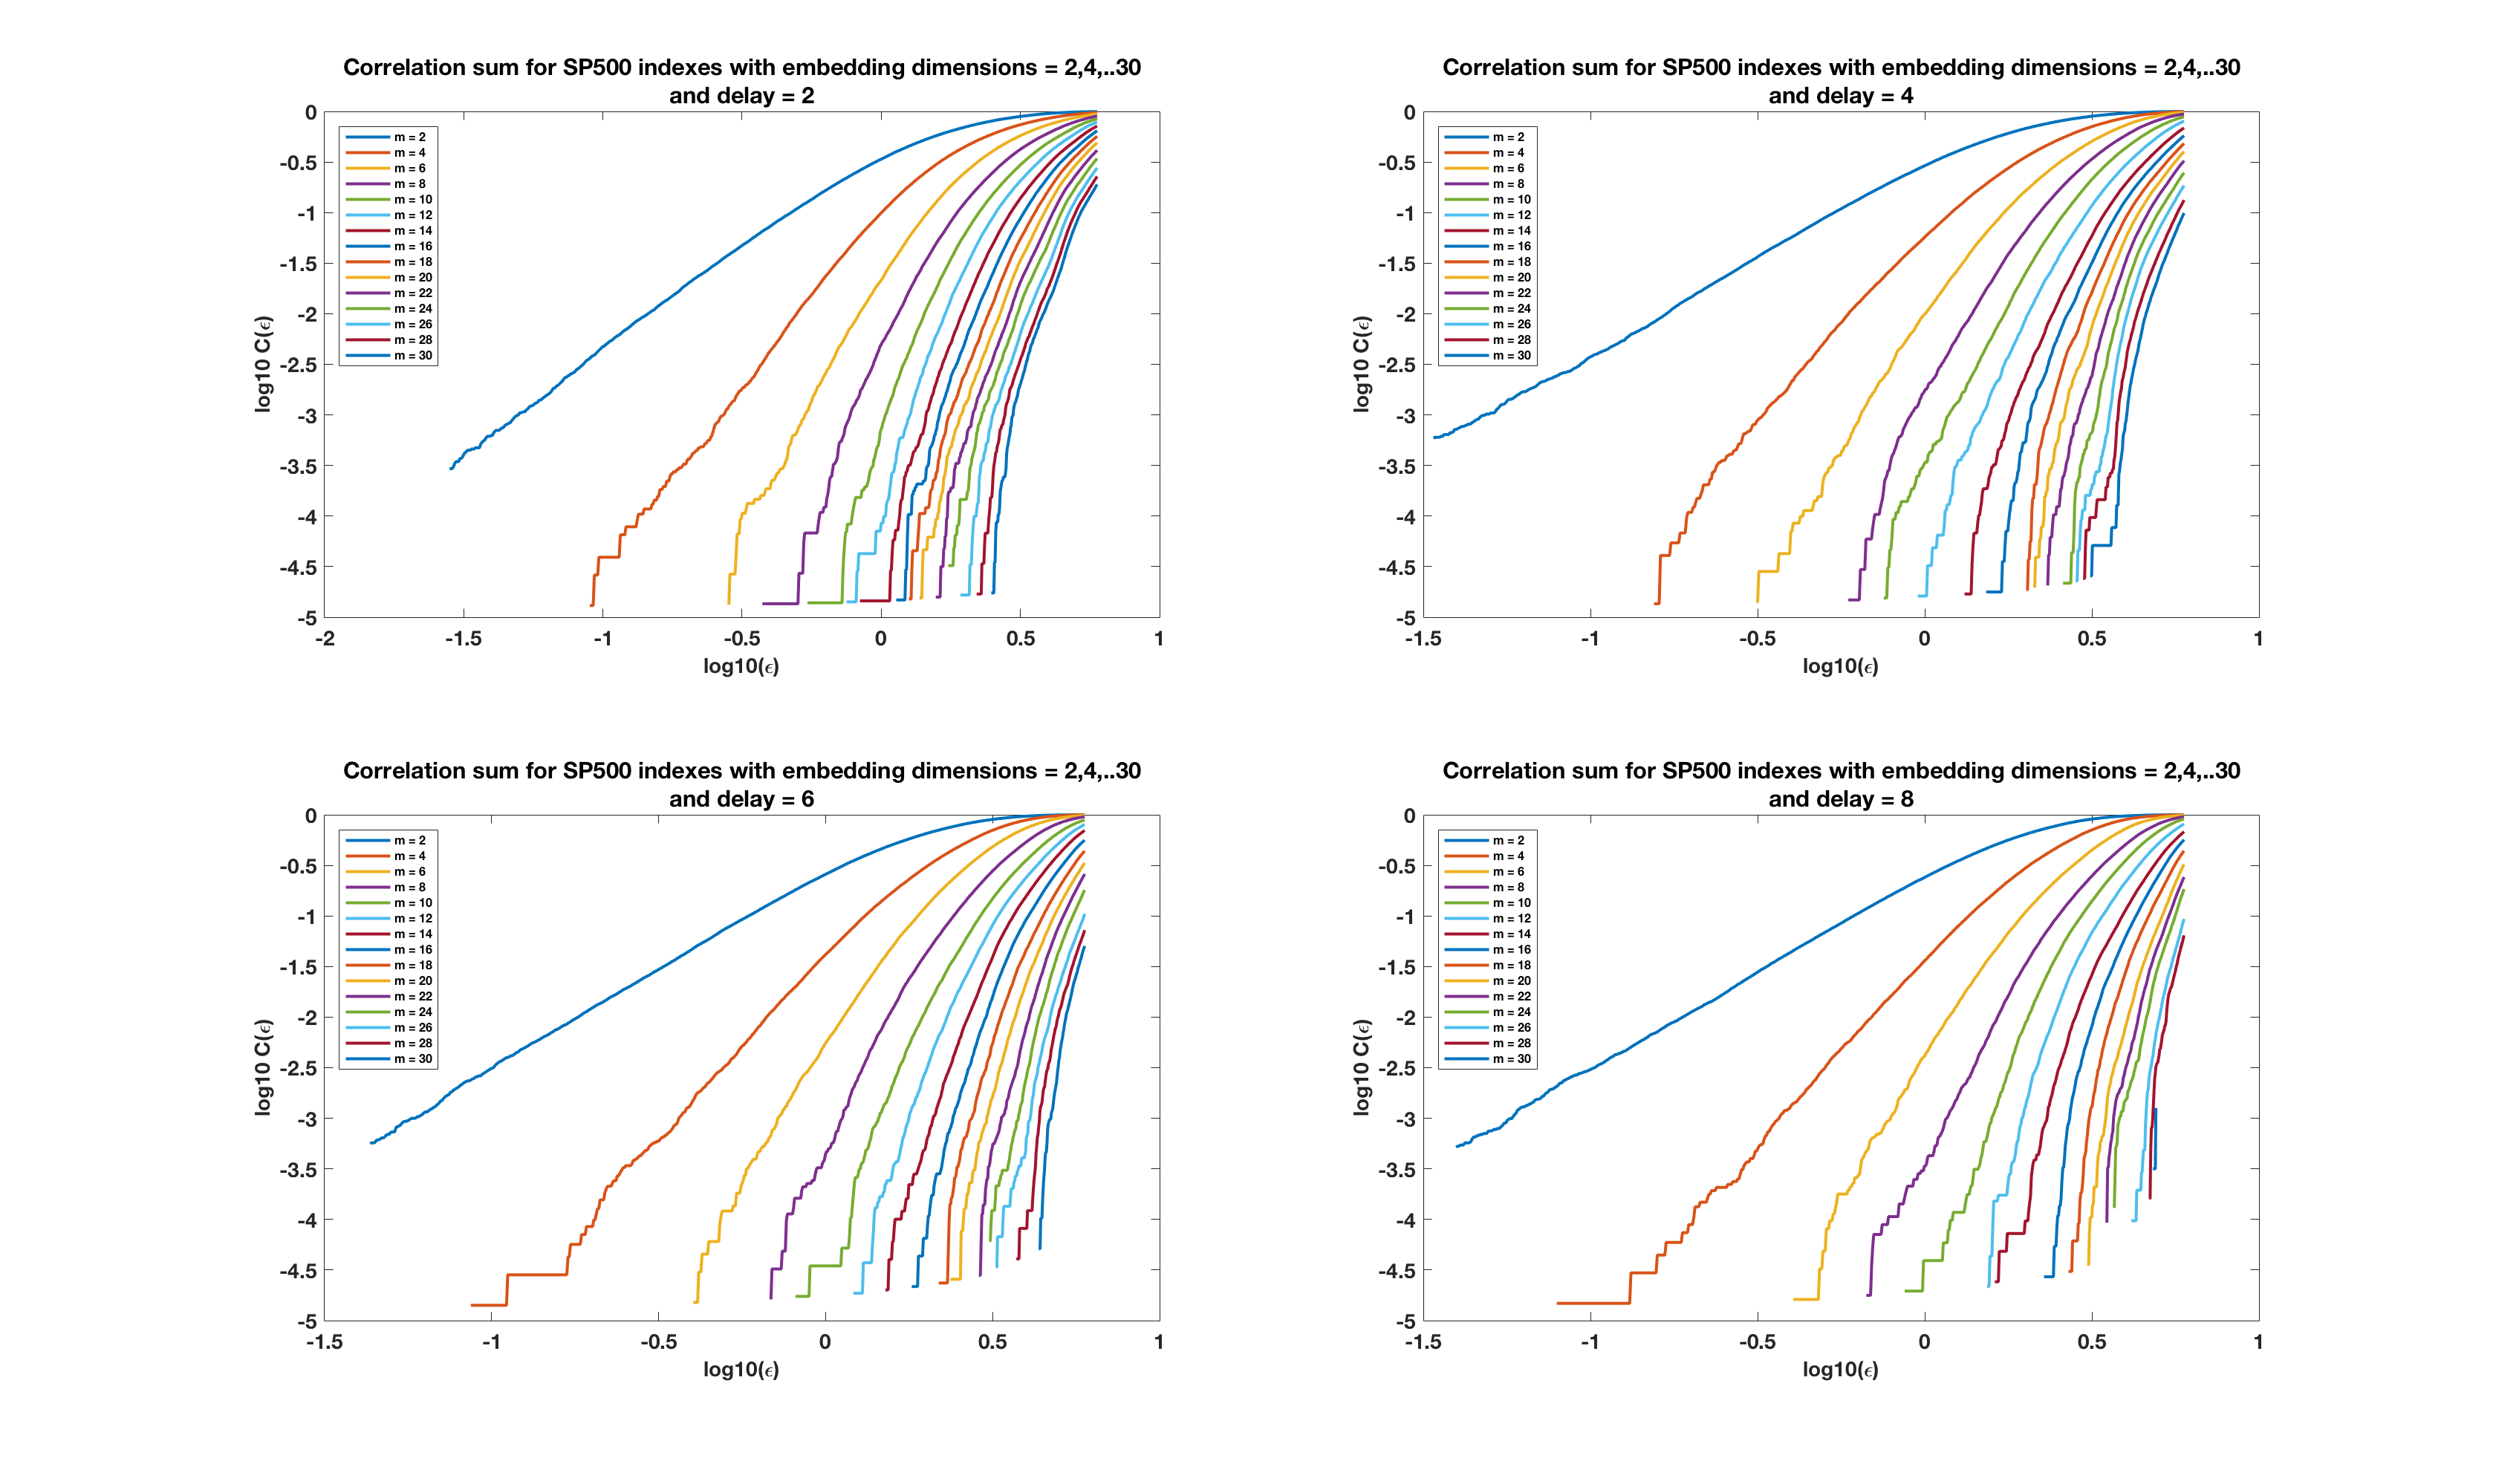
\includegraphics[scale=.15]{Images/SP500CD1}
\caption{Correlation Dimension for NASDAQ. The graph was created by using drawCorrDim.m and it is attached in the Appendix}
\label{fig:SP500CD1}
\end{figure}

\begin{figure}[!ht]
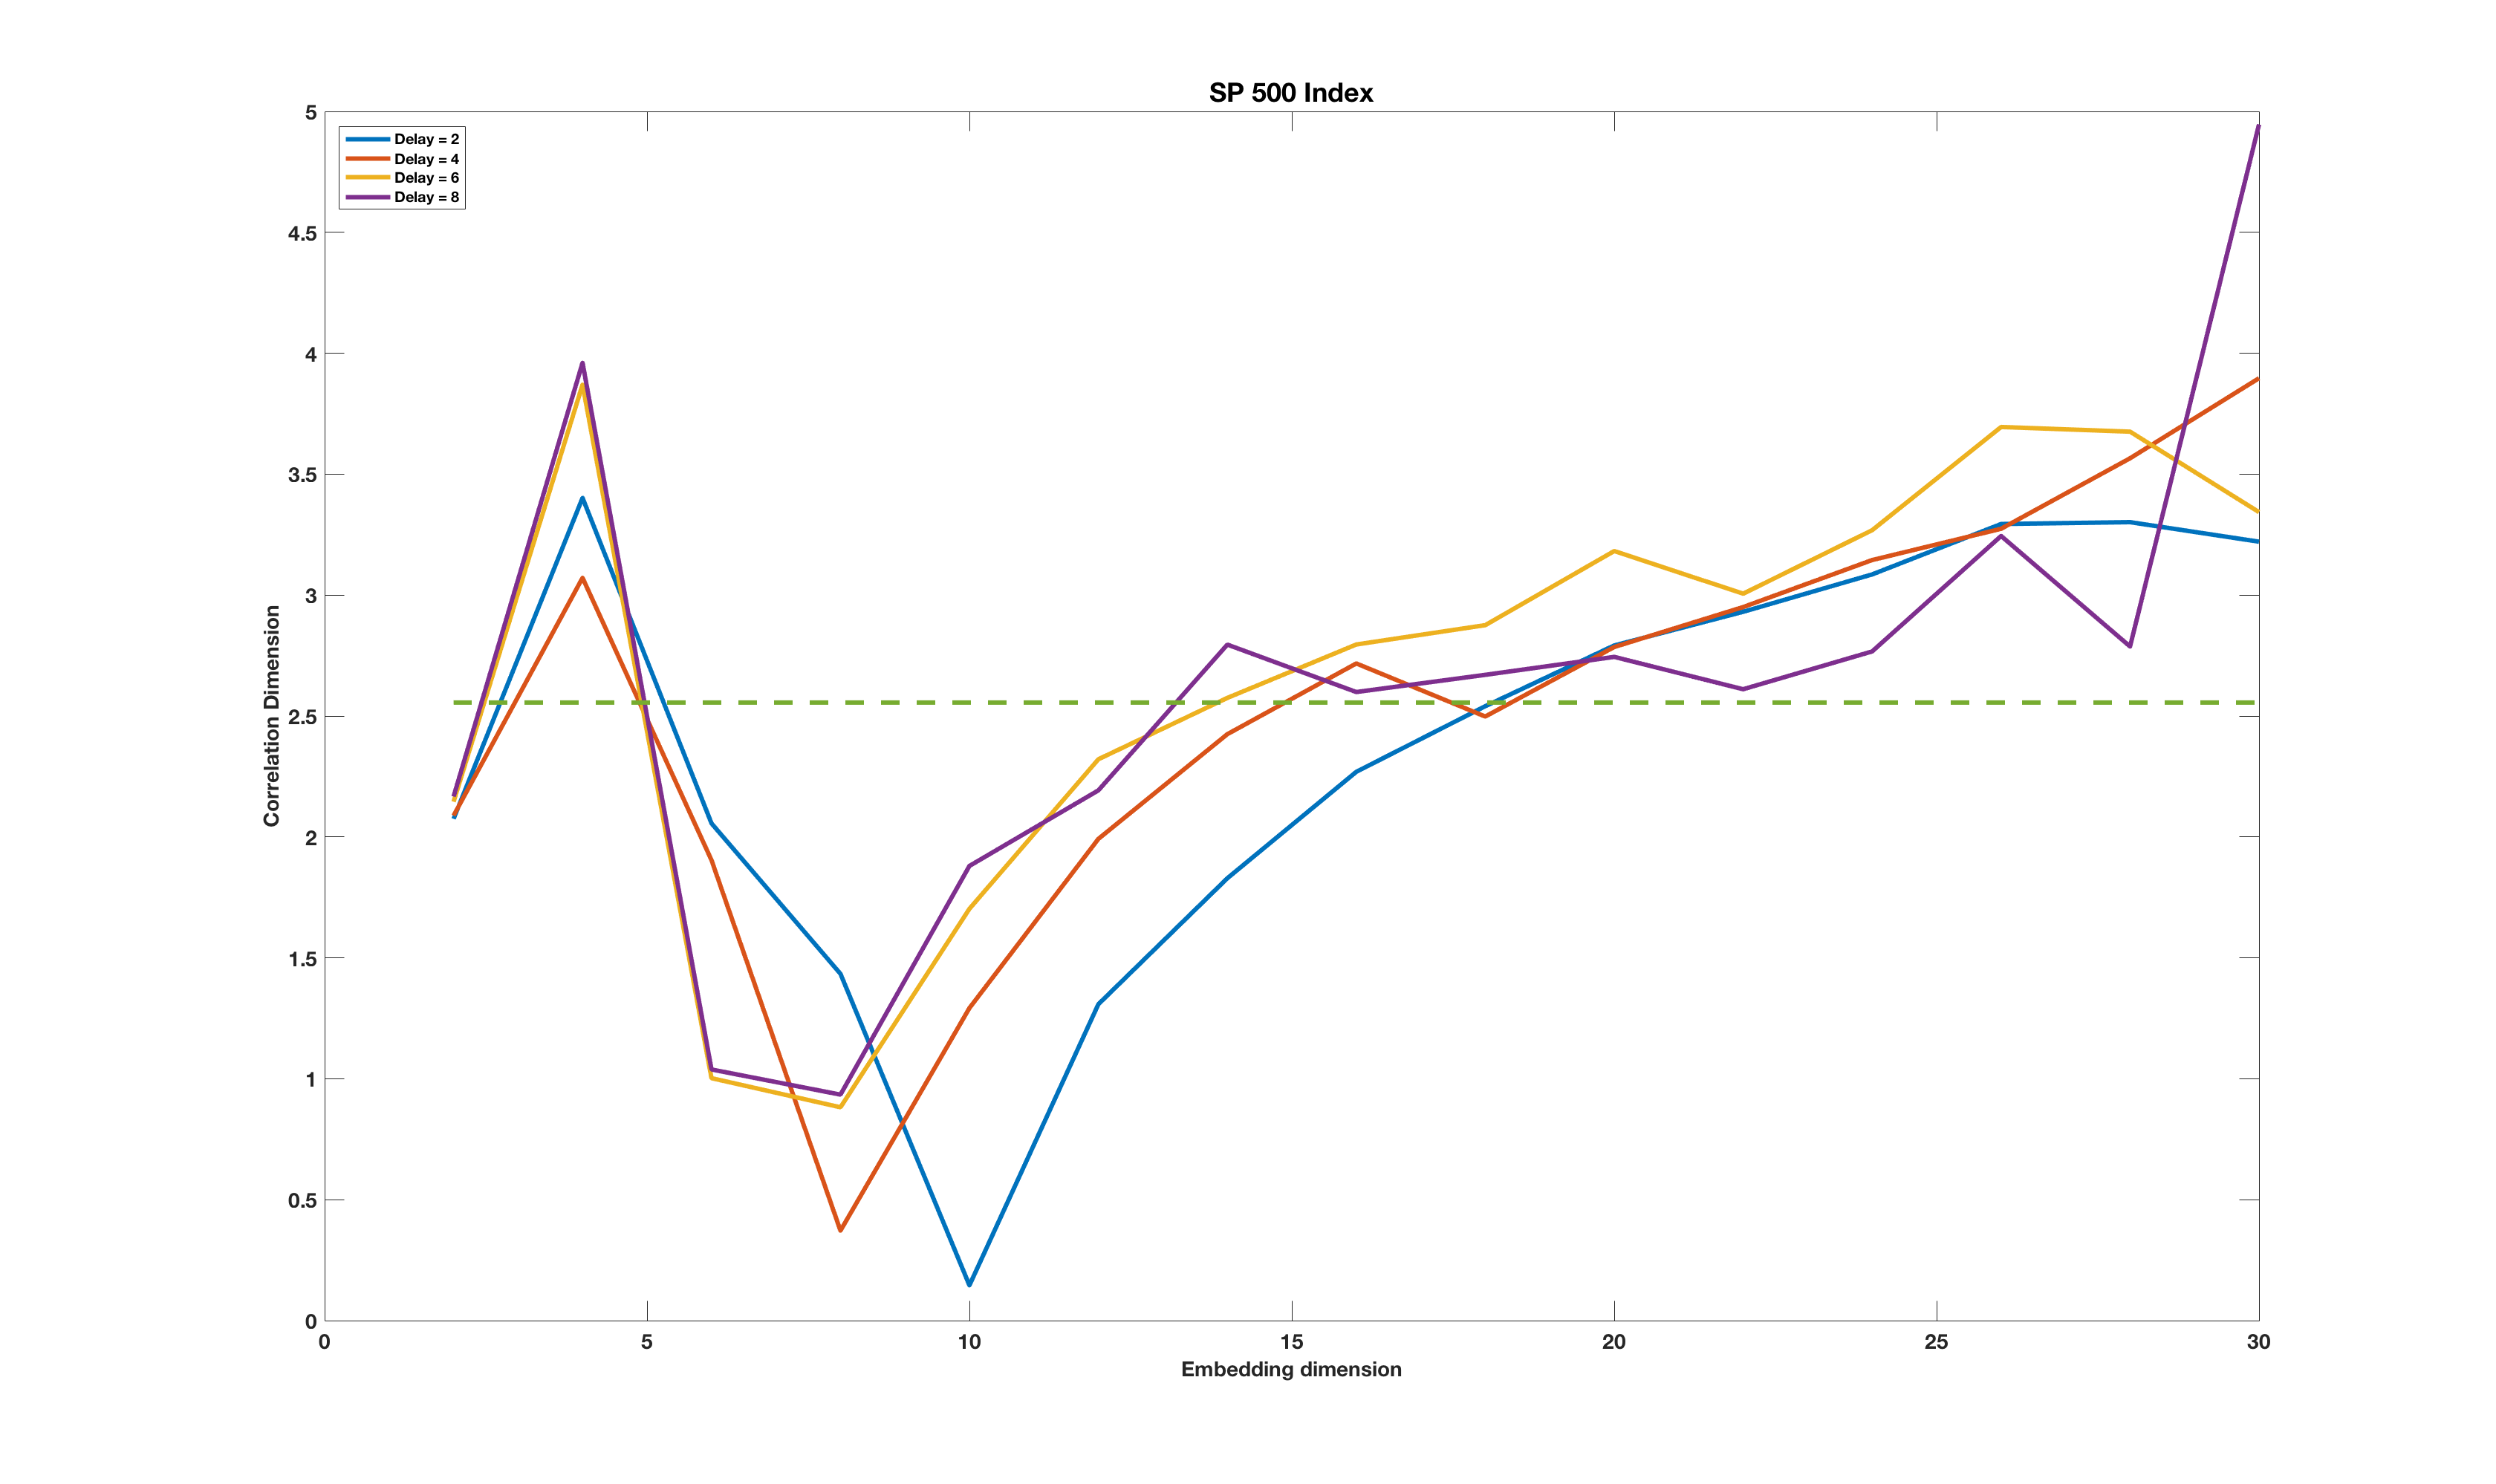
\includegraphics[scale=.15]{Images/SP500CD2}
\caption{Correlation Dimension for NASDAQ. The graph was created by using drawCorrDim.m and it is attached in the Appendix}
\label{fig:SP500CD2}
\end{figure}

\begin{figure}[!ht]
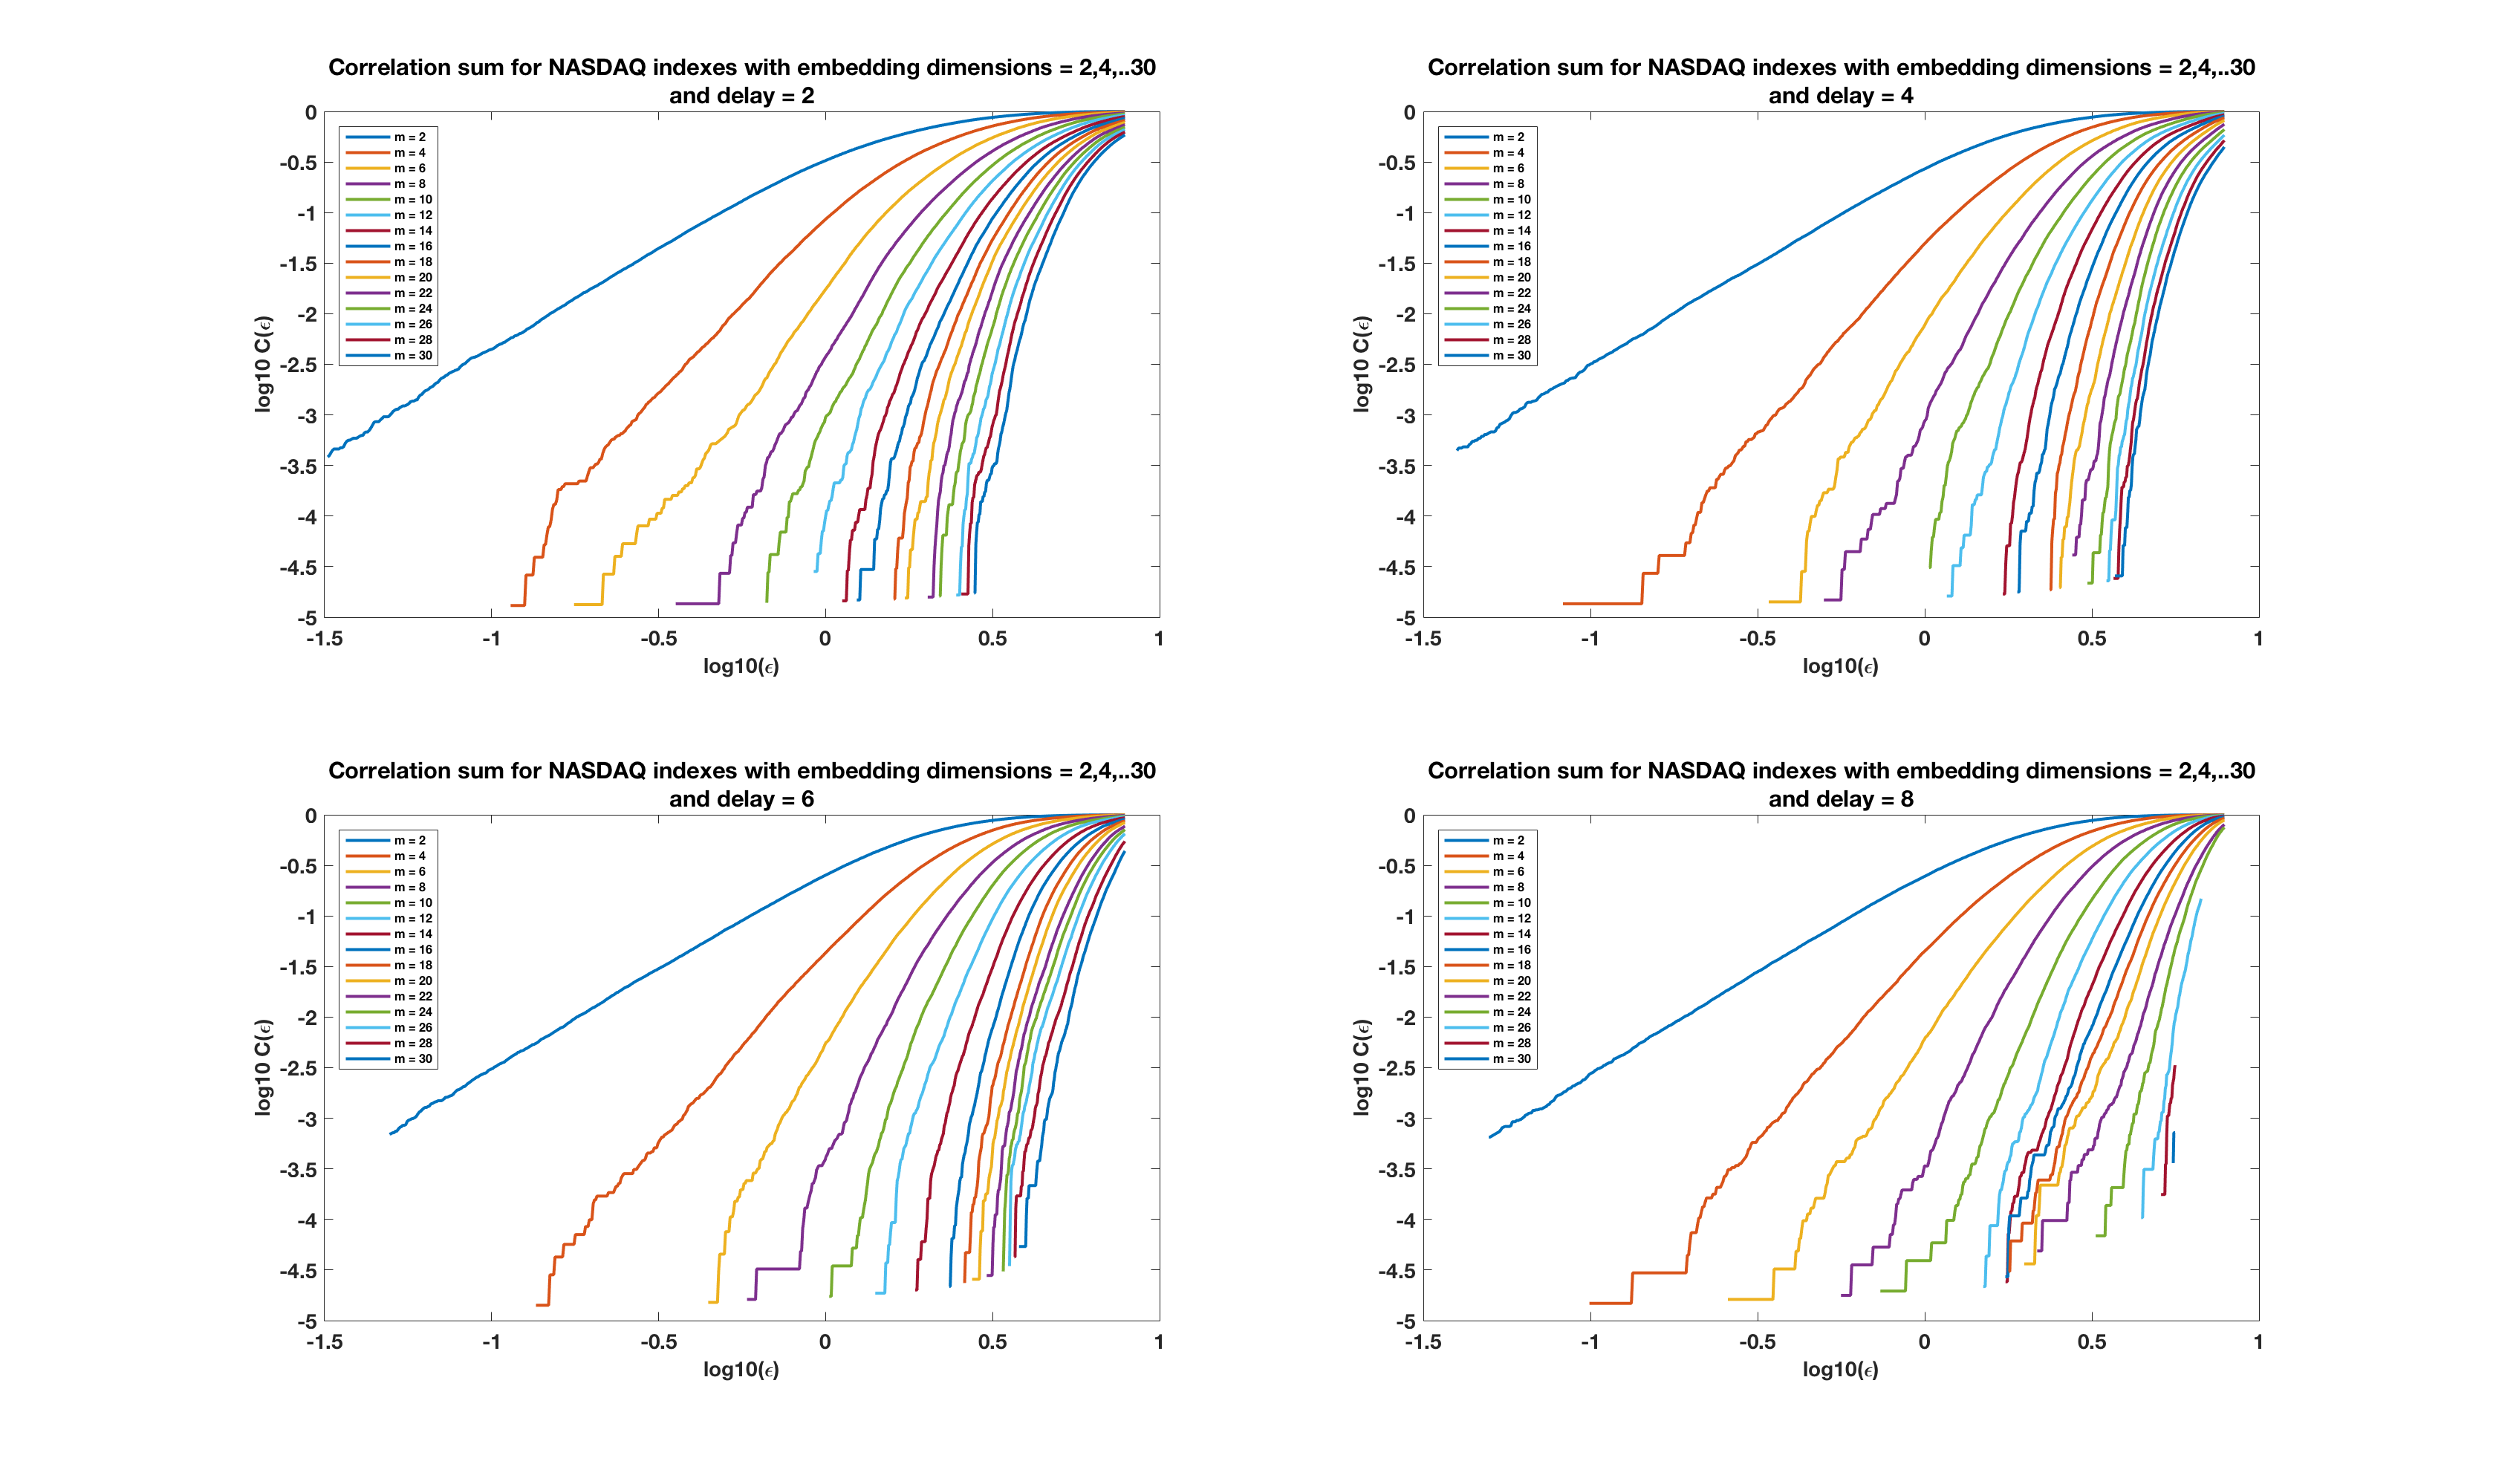
\includegraphics[scale=.15]{Images/NASDAQCD1}
\caption{Correlation Dimension for NASDAQ. The graph was created by using drawCorrDim.m and it is attached in the Appendix}
\label{fig:NASDAQCD1}
\end{figure}

\begin{figure}[!ht]
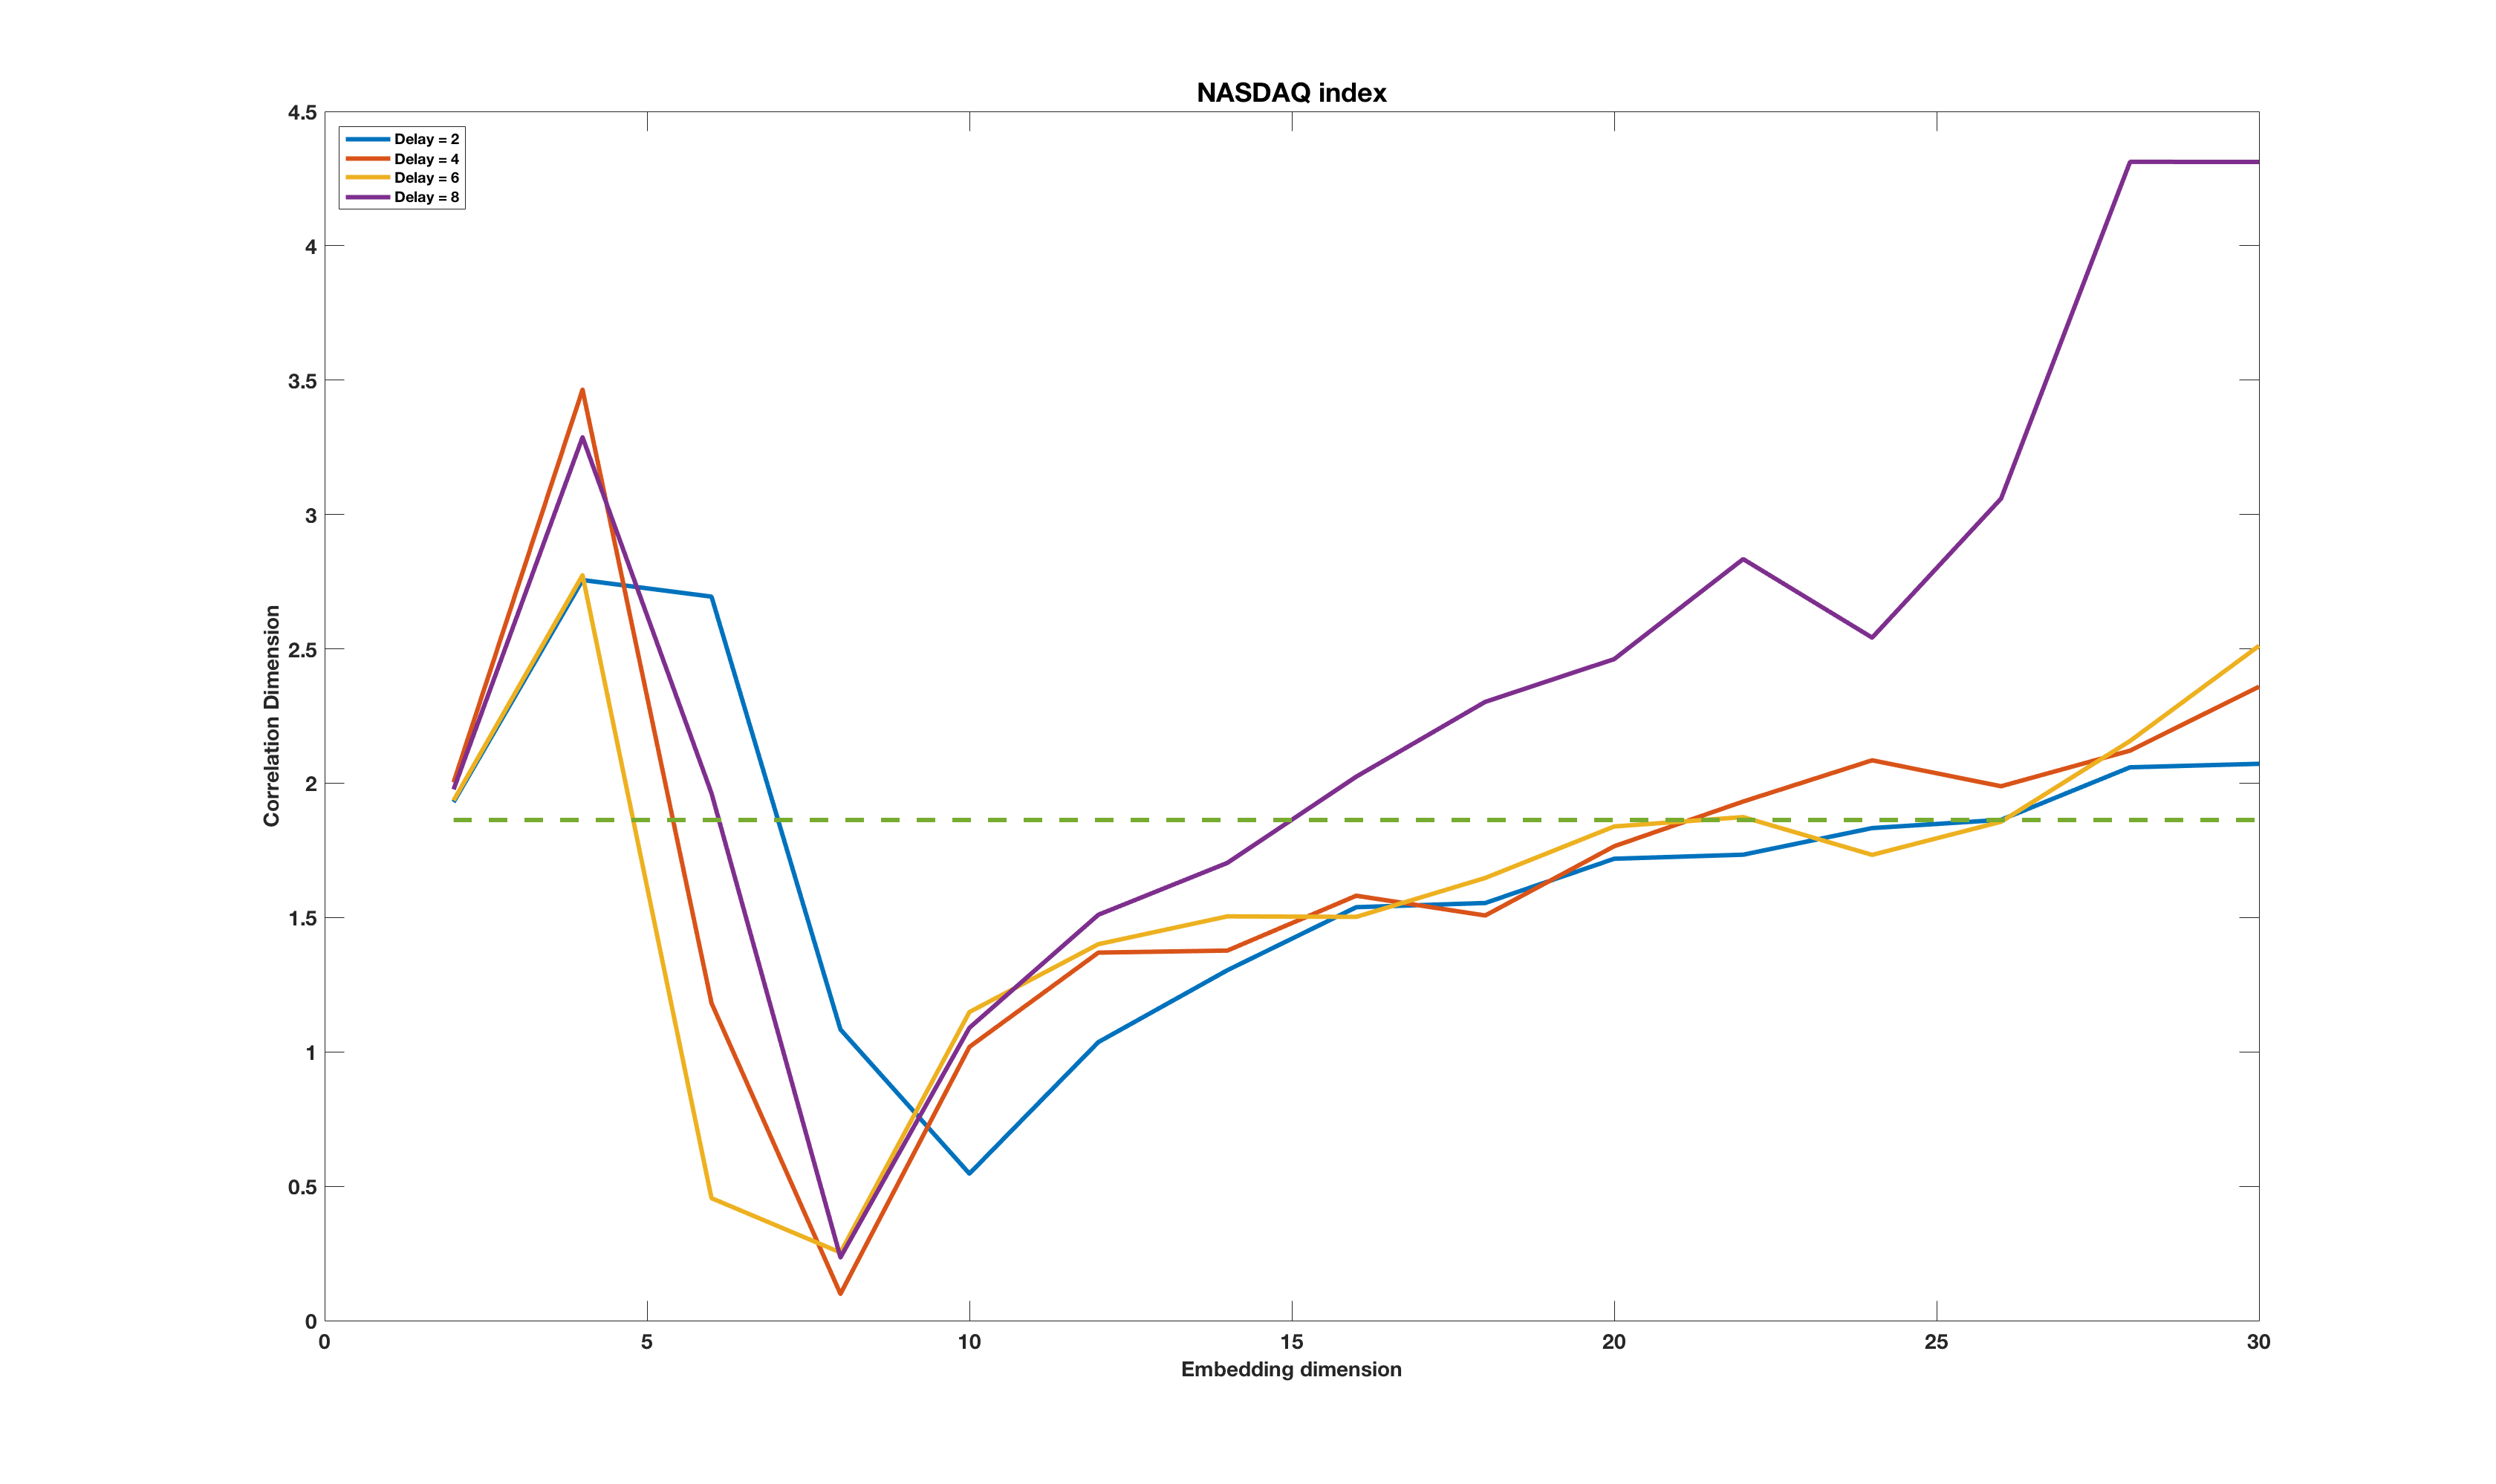
\includegraphics[scale=.15]{Images/NASDAQCD2}
\caption{Correlation Dimension for NASDAQ. The graph was created by using drawCorrDim.m and it is attached in the Appendix}
\label{fig:NASDAQCD2}
\end{figure}



\subsection{Lyapunov exponent}
The Lyapunov exponent is a quantity that describes the rate of separation of two neighbouring trajectories. The divergence of two trajectories at time $t$ with initial separation $\delta Z_0$ at $t=0$, is expressed as:

\begin{equation} \label{le:1}
|\delta Z(t)| \approx e^{\lambda t}|\delta Z_0|
\end{equation}
where $\lambda$ is the Lyapunov exponent. Different orientations of initial separation vectors would result in different rate of separation and thus, a whole spectrum of the Lyapunov exponents. The Largest $\lambda$ is called the Maximum Lyapunov Exponent: 

\begin{equation} \label{le:2}
%\lambda = lim_{t\to\infy} \frac{1}{t}
D_c = \lim_{\epsilon\to 0} \lim_{N\to\infty} \frac{\partial log_{10} C(\epsilon)}{\partial log_{10}(\epsilon)}
\end{equation}

%\lambda = lim_{t\to\infy} \frac{1}{t} ln \frac{|\delta Z(t)}|{\delta Z_0}

$\lambda gt 0$ is usually considered as indicator of chaos, $\lambda lt 0$ is usually considered an indicator of a mean reverting behavior and $\lambda = 0$ is a characteristic of cyclic behavior. 

\subsection{Instantaneous Autocorrelations and instantaneous frequency in Time-frequency representation}

The concepts of instantaneous autocorrelation and instantaneous frequency are important in developing generalized spectral analysis. A symmetric window in a localized time interval is introduced in the instantaneous autocorrelation function of the bilinear Wigner distribution (WD); the corresponding time-dependent frequency (or simply time frequency) can be defined by the Fourier spectrum of its autocorrelations. 

\begin{figure}[!ht]
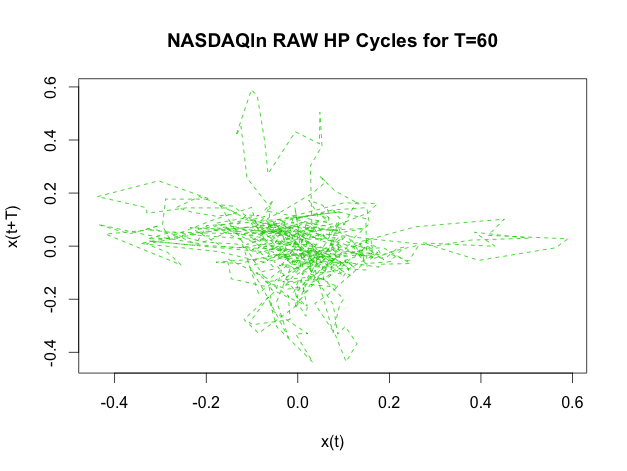
\includegraphics[scale=.7]{Images/NASDAQRawChaos}
\caption{Phase Portrait for log(NASDAQ) unfiltered series $T= 60$. The graph was created by using Attractor.R (R program) and it is attached in the Appendix A}
\label{fig:NASDAQRawChaos}
\end{figure}

\begin{figure}[!ht]
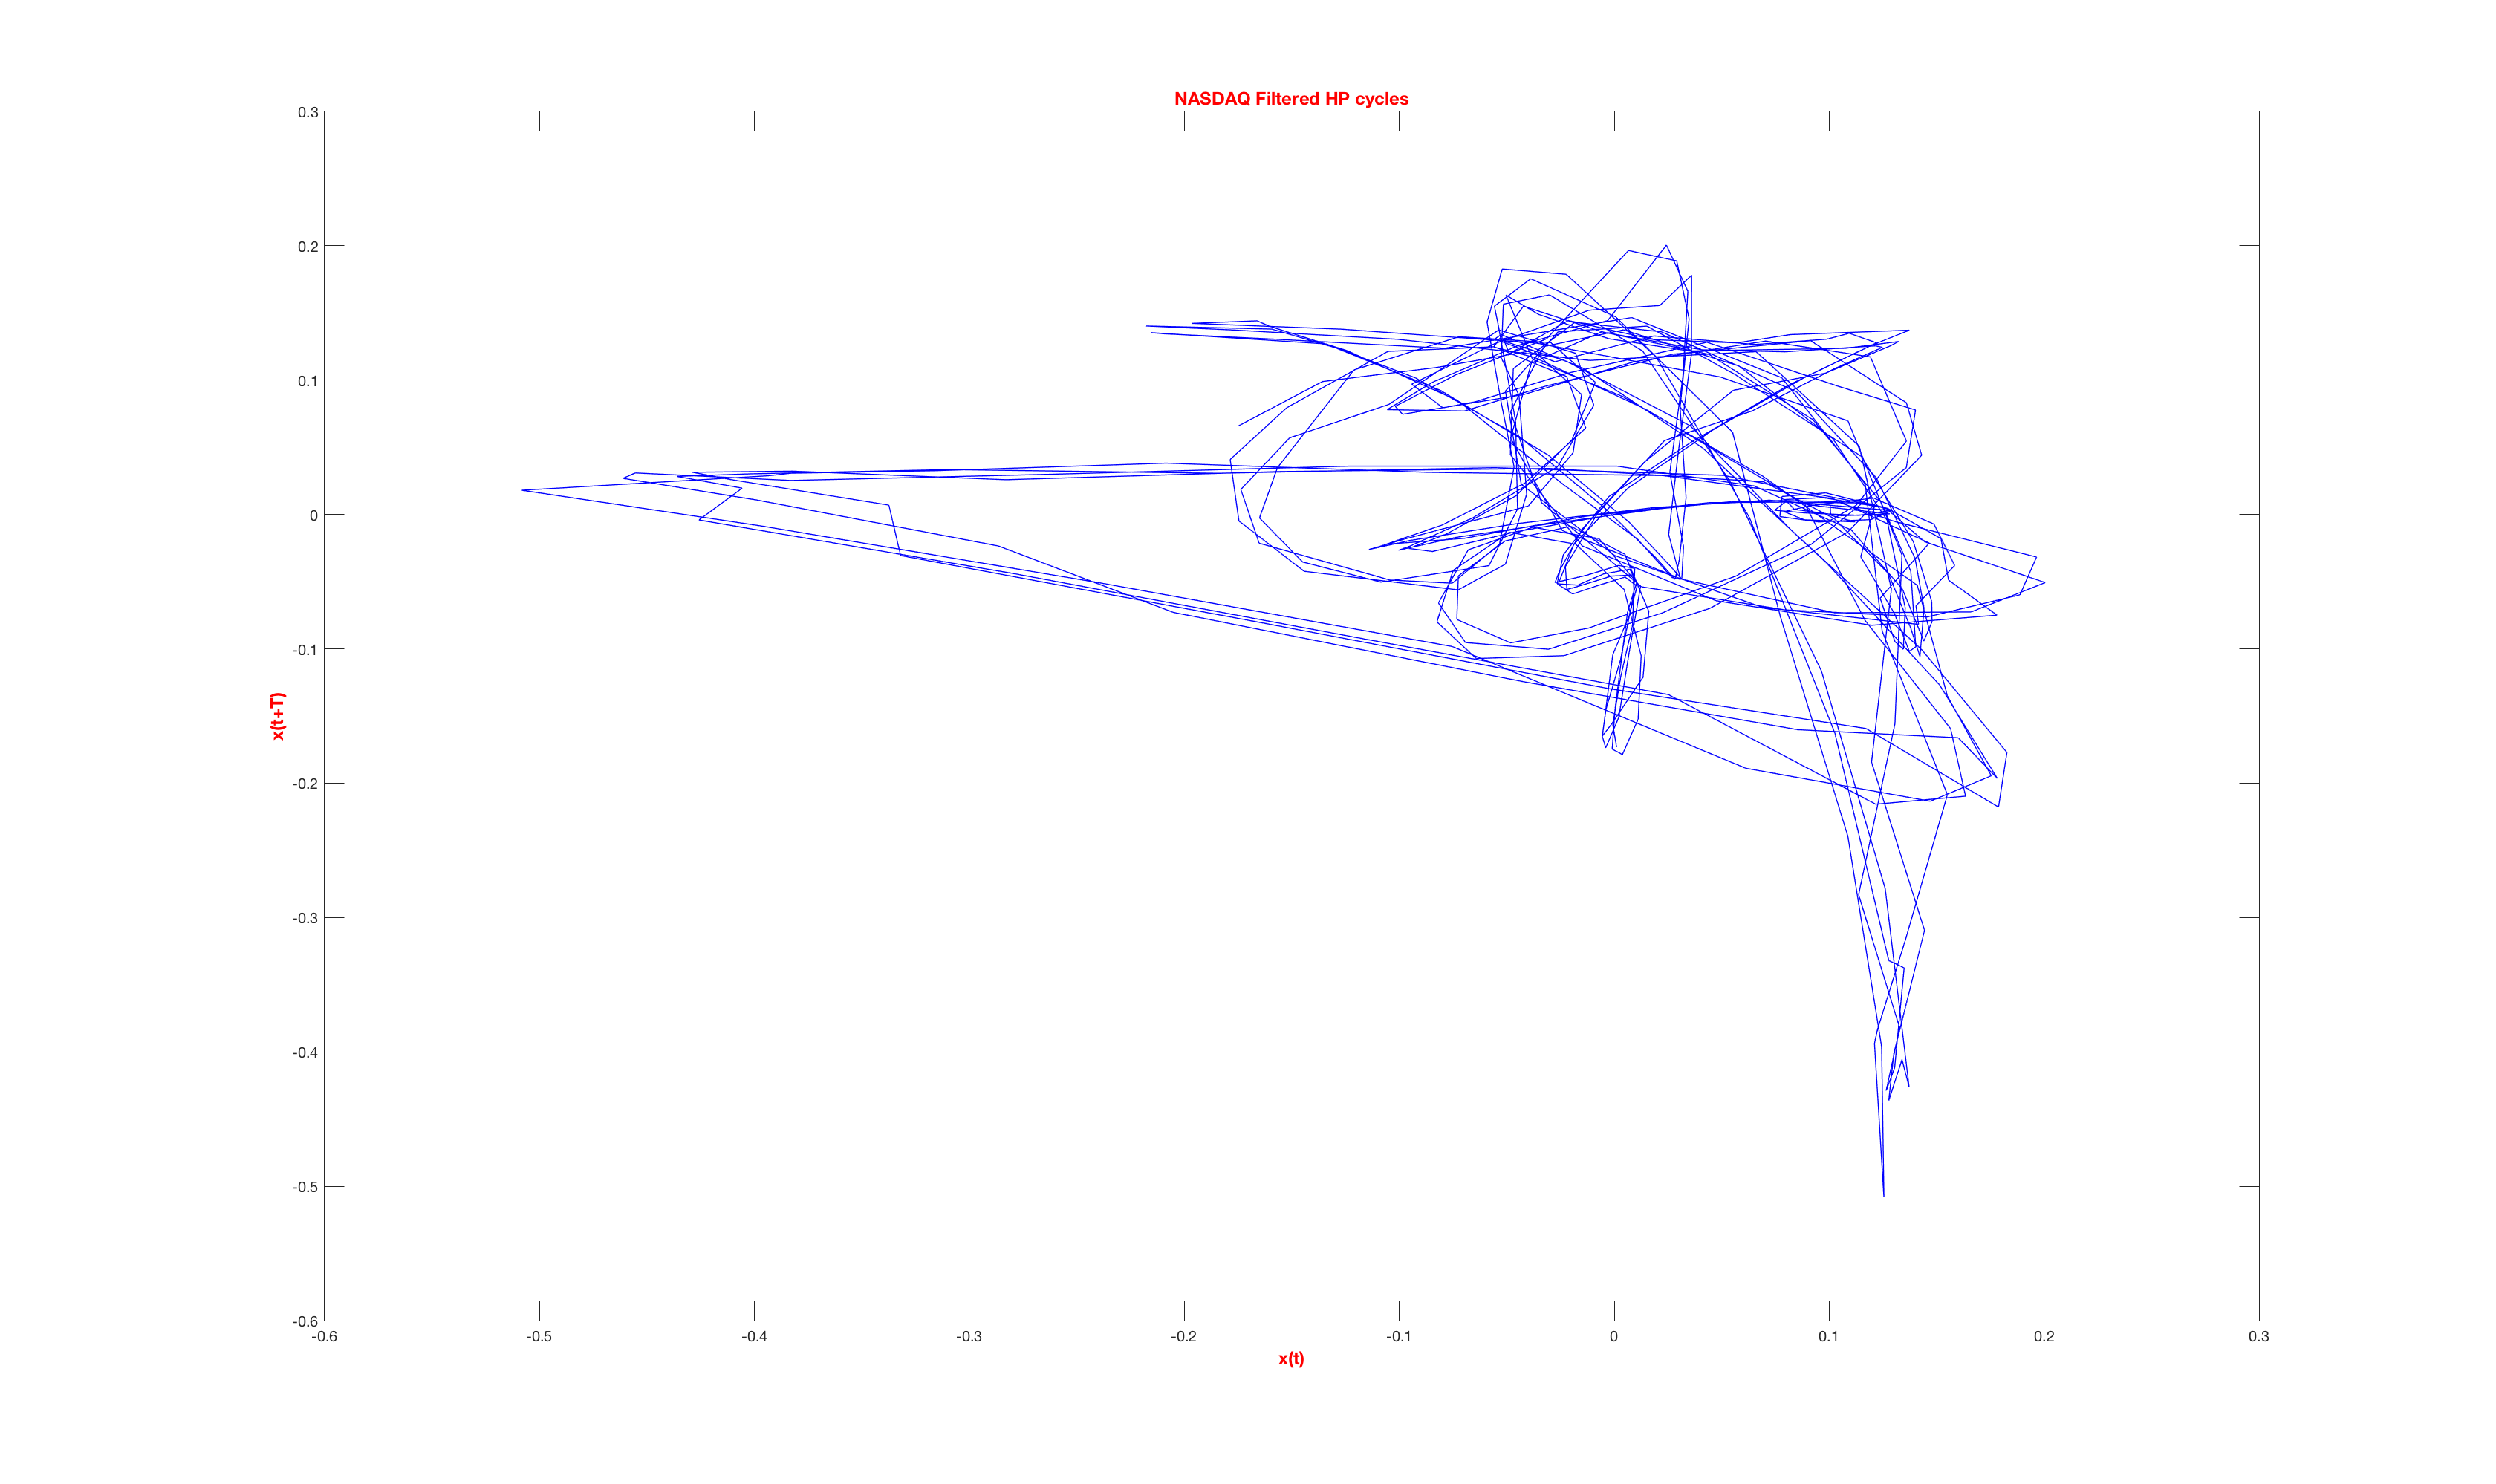
\includegraphics[scale=.15]{Images/NASFiltAttract}
\caption{Phase Portrait for log(NASDAQ) unfiltered series $T= 60$. A pattern of strange attractor can be observed in the graph. The threshold value that depends on $H$ $(H = 0.5)$ has less significant impact to the pattern emergence whereas the size of $m$, $n$ in $C(m,n)$, the Gabor Coefficient has significant impact to the pattern of strange attractor. The $16 x 16$ Gabor Coefficient was used. The graph was created by using myAttractor.m (Matlab program) and it is attached in the Appendix B.}
\label{fig:NASFiltAttract}
\end{figure}

\begin{figure}[!ht]
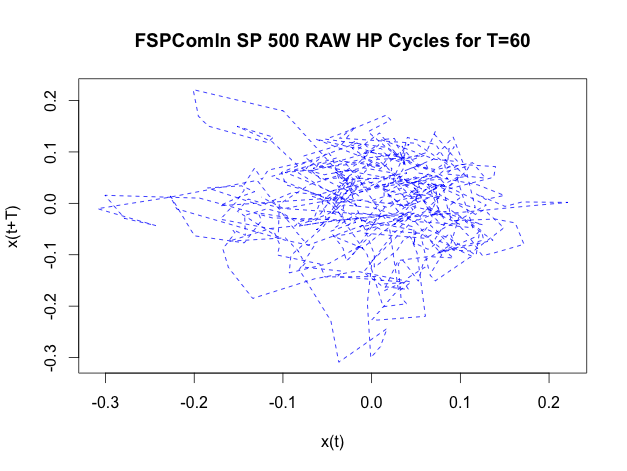
\includegraphics[scale=.7]{Images/SP500RawChaos}
\caption{Phase Portrait for log(SP500) unfiltered series $T= 60$. The graph was created by using Attractor.R (R program) and it is attached in the Appendix A.}
\label{fig:SP500RawChaos}
\end{figure}

\begin{figure}[!ht]
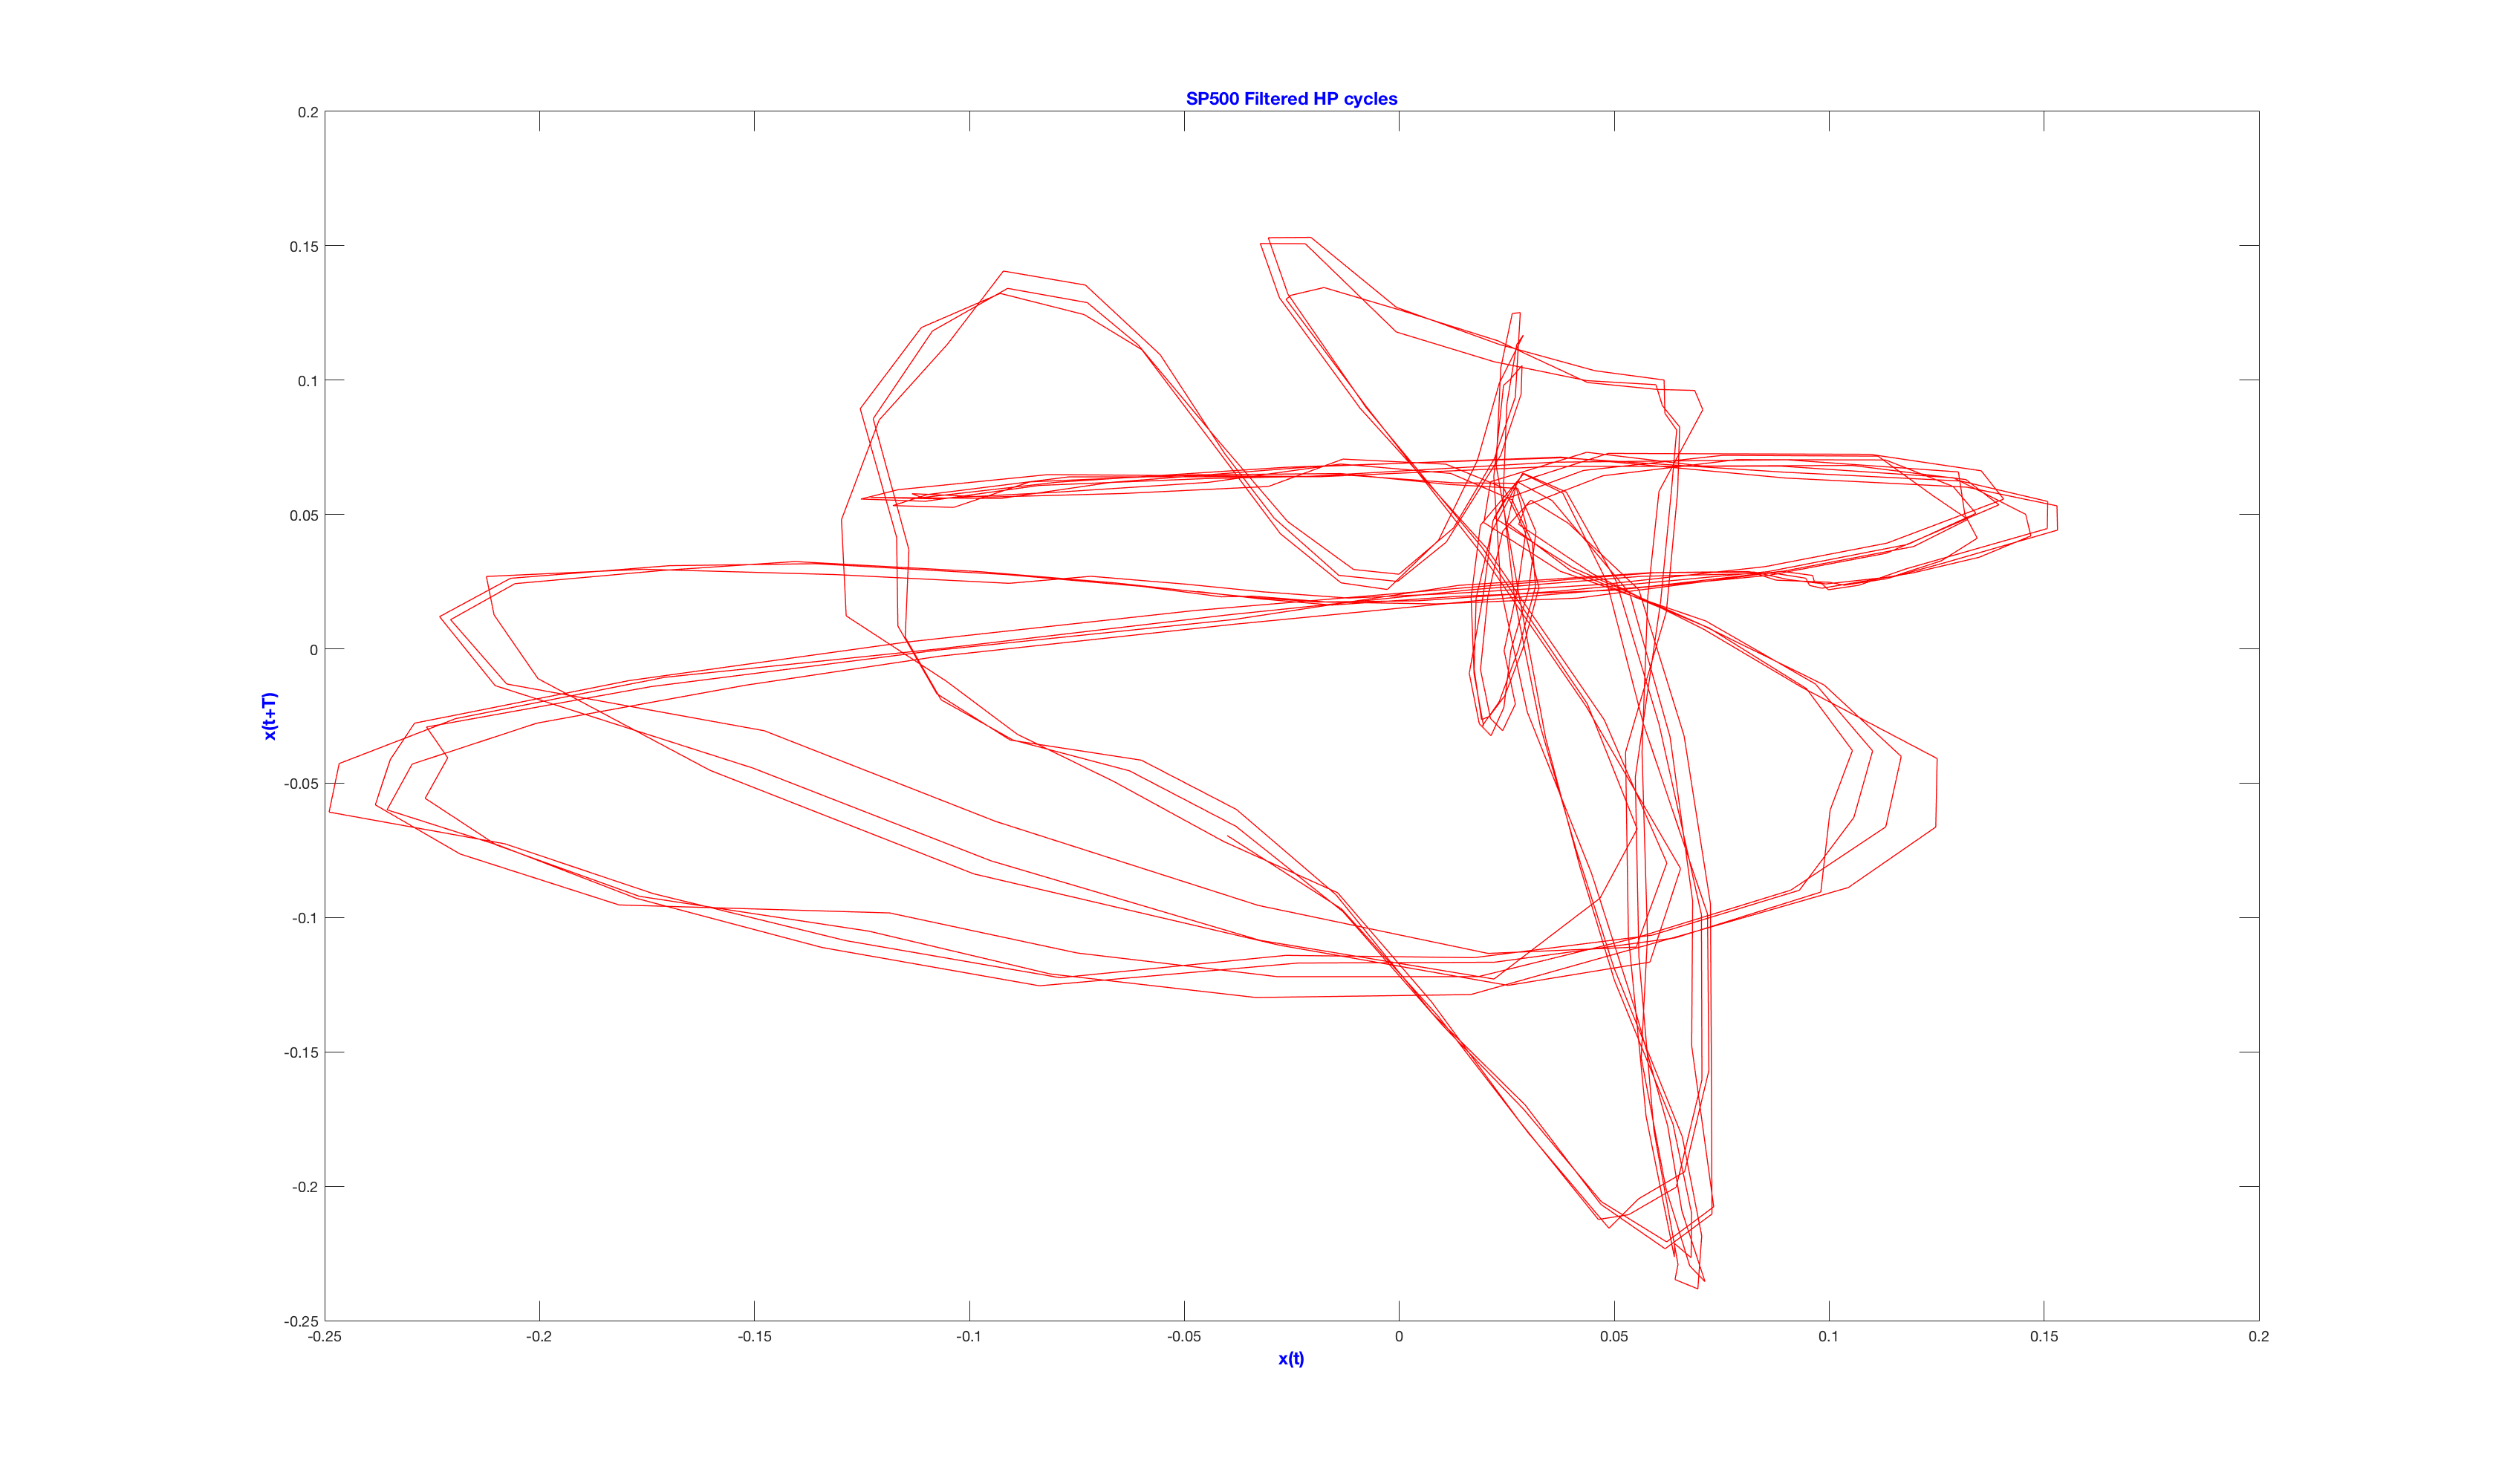
\includegraphics[scale=.15]{Images/SPFiltAttract}
\caption{Phase Portrait for log(SP500) unfiltered series $T= 60$. A pattern of strange attractor can be observed in the graph. The threshold value that depends on $H$ $(H = 0.5)$ has less significant impact to the pattern emergence whereas the size of $m$, $n$ in $C(m,n)$, the Gabor Coefficient has significant impact to the pattern of strange attractor. The $16 x 16$ Gabor Coefficient was used. The graph was created by using myAttractor.m (Matlab program) and it is attached in the Appendix B.}
\label{fig:SPFiltAttract}
\end{figure}

In the figure ~\ref{fig:SP500RawChaos} the chaos of the SP500 is shown and in the figure ~\ref{fig:NASDAQRawChaos} the chaos of the SP500 is shown.


\begin{figure}[!ht]
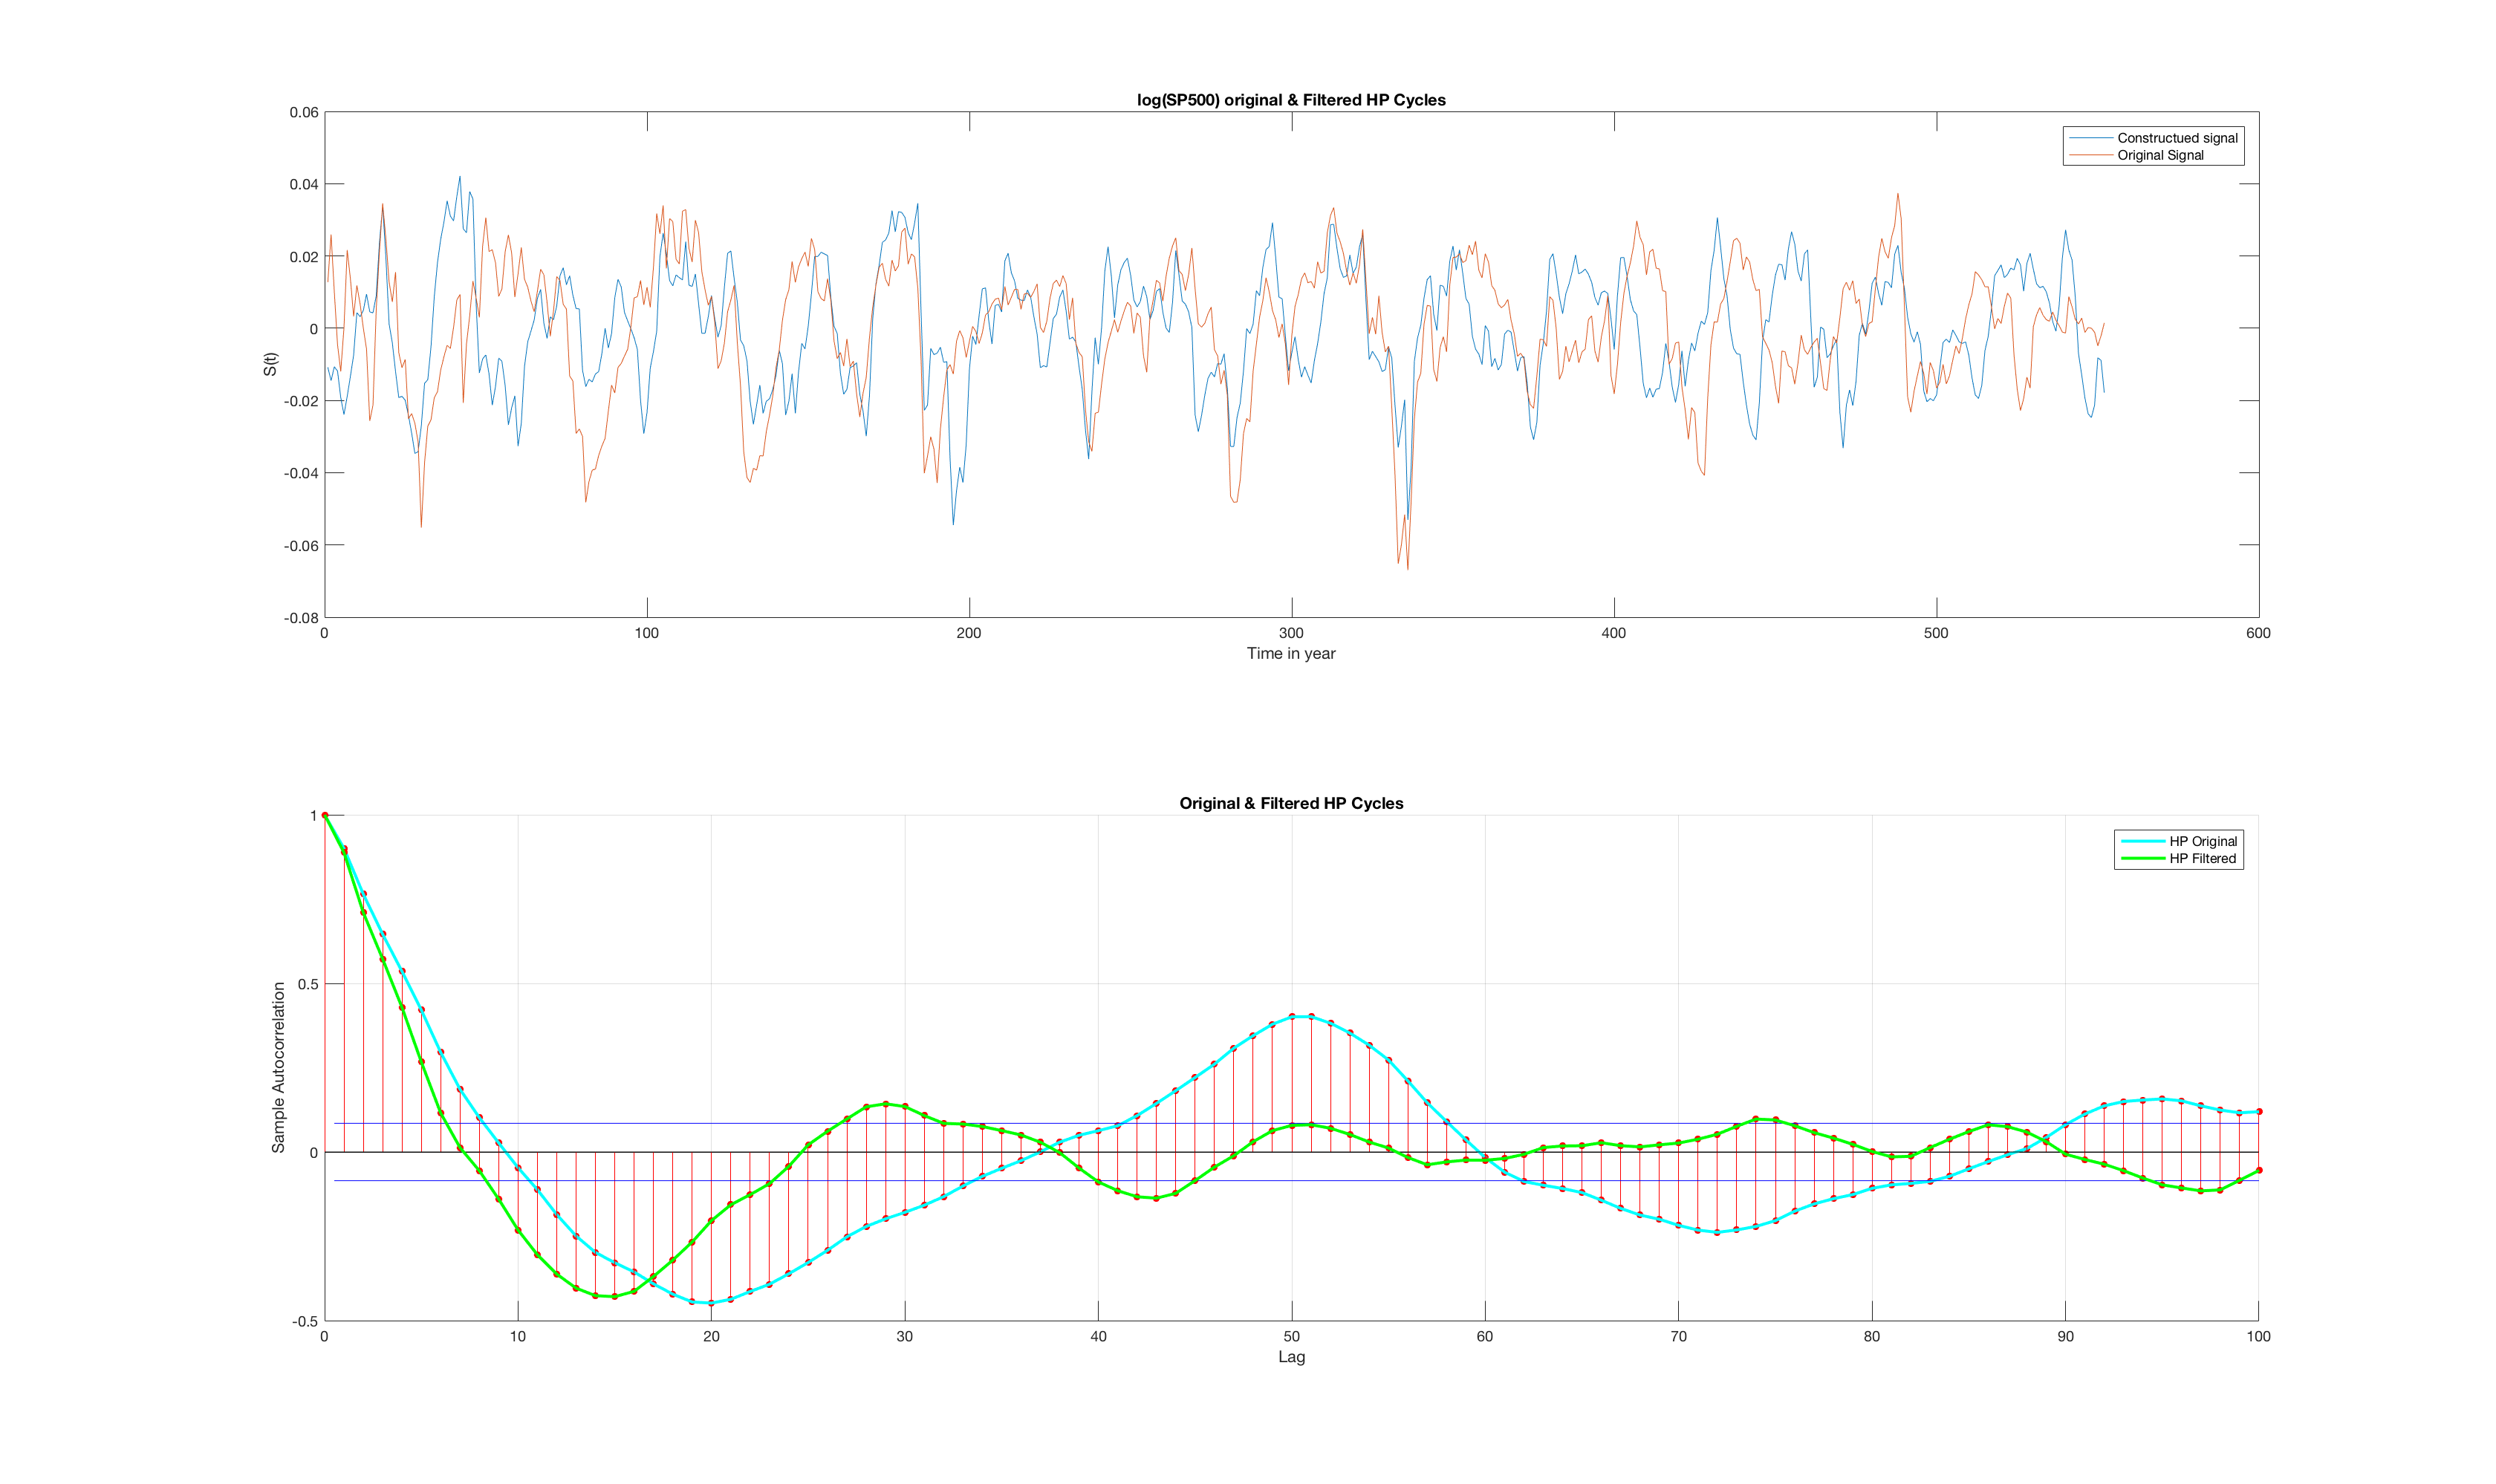
\includegraphics[scale=.15]{Images/SP500Recon}
\caption{Fig a) The original and reconstructed time series of log(SP500) HP Cycles. Gabor Coefficients are created using the parameters - .$\Delta M = 8; \Delta N = 4; m = 16; n = 16; \sigma = \sqrt{\frac{\Delta M L}{\Delta N 2\pi}}$. Fig b) Autocorelations of the original and reconstructed time series of log(SP500) HP cycle. The program used to create the graph is myreconstfromgabor.m and it is attached in the appendix B.}
\label{fig:SP500Recon}
\end{figure}

\begin{figure}[!ht]
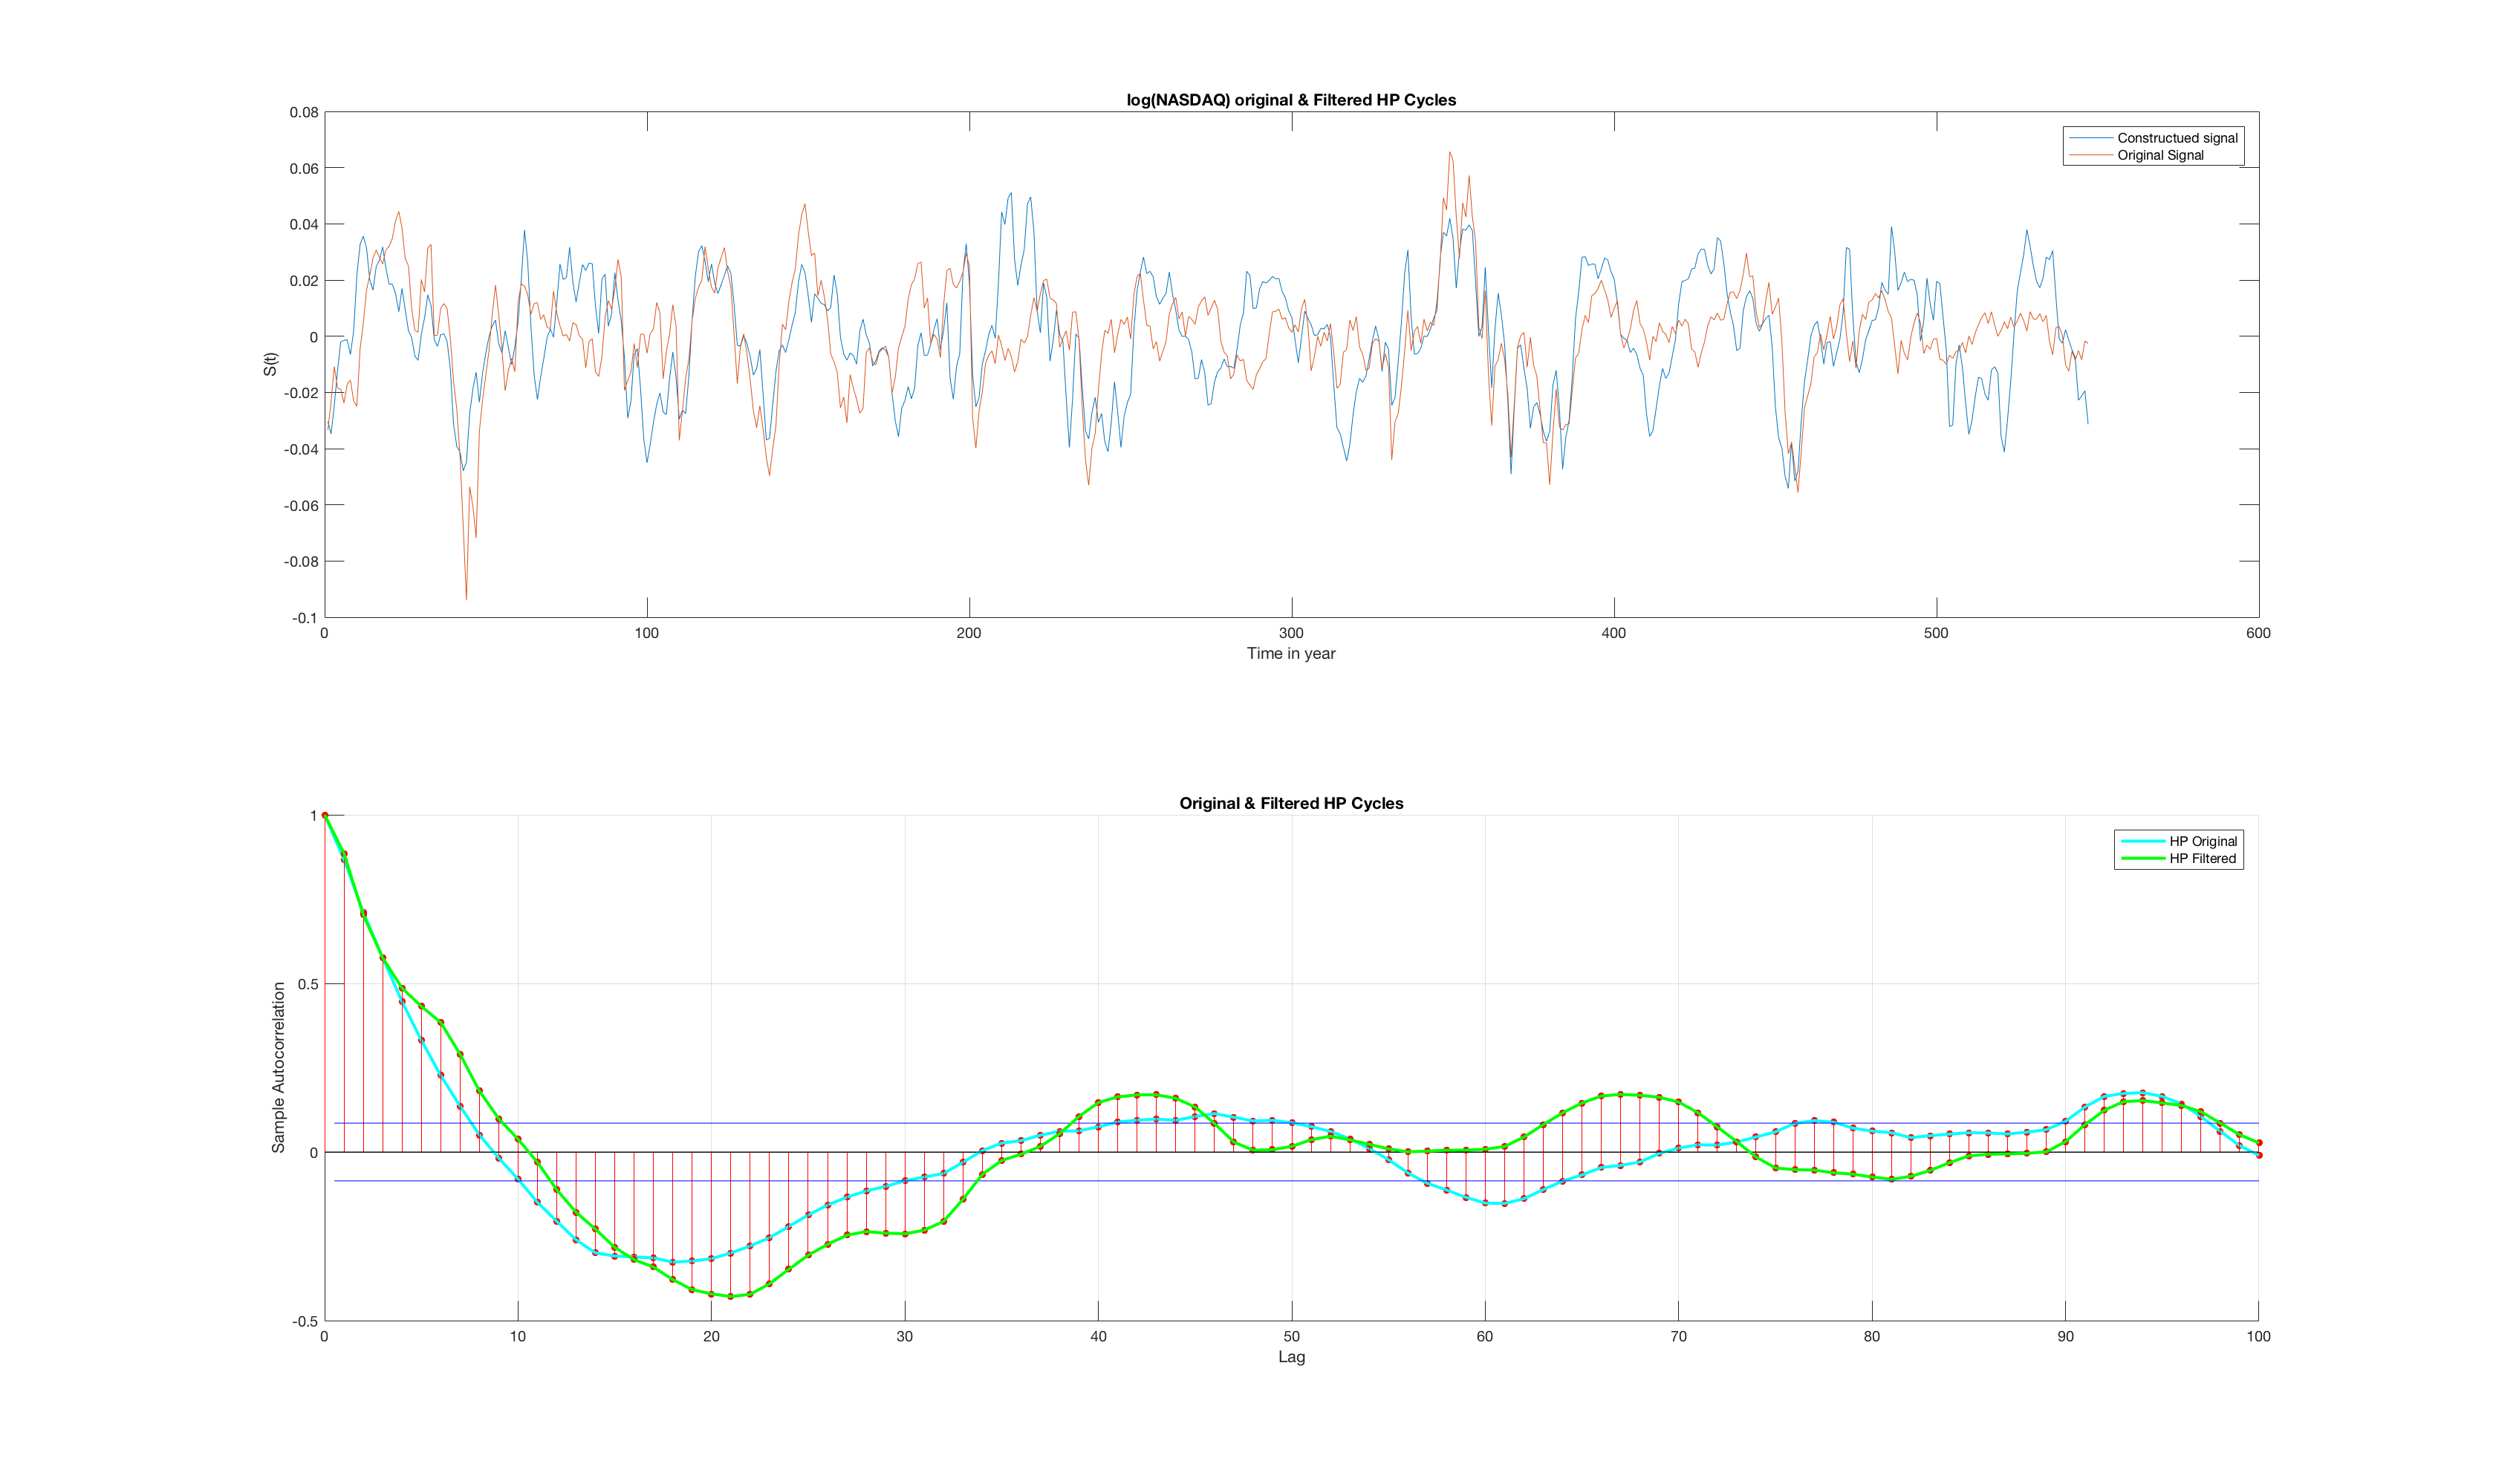
\includegraphics[scale=.15]{Images/NASRecon}
\caption{Fig a) The original and reconstructed time series of log(NASDAQ) HP Cycles. Gabor Coefficients are created using the parameters - .$\Delta M = 8; \Delta N = 4; m = 16; n = 16; \sigma = \sqrt{\frac{\Delta M L}{\Delta N 2\pi}}$. Fig b) Autocorelations of the original and reconstructed time series of log(NASDAQ) HP cycle. The program used to create the graph is myreconstfromgabor.m and it is attached in the appendix B.}
\label{fig:NASRecon}
\end{figure}

\begin{figure}[!ht]
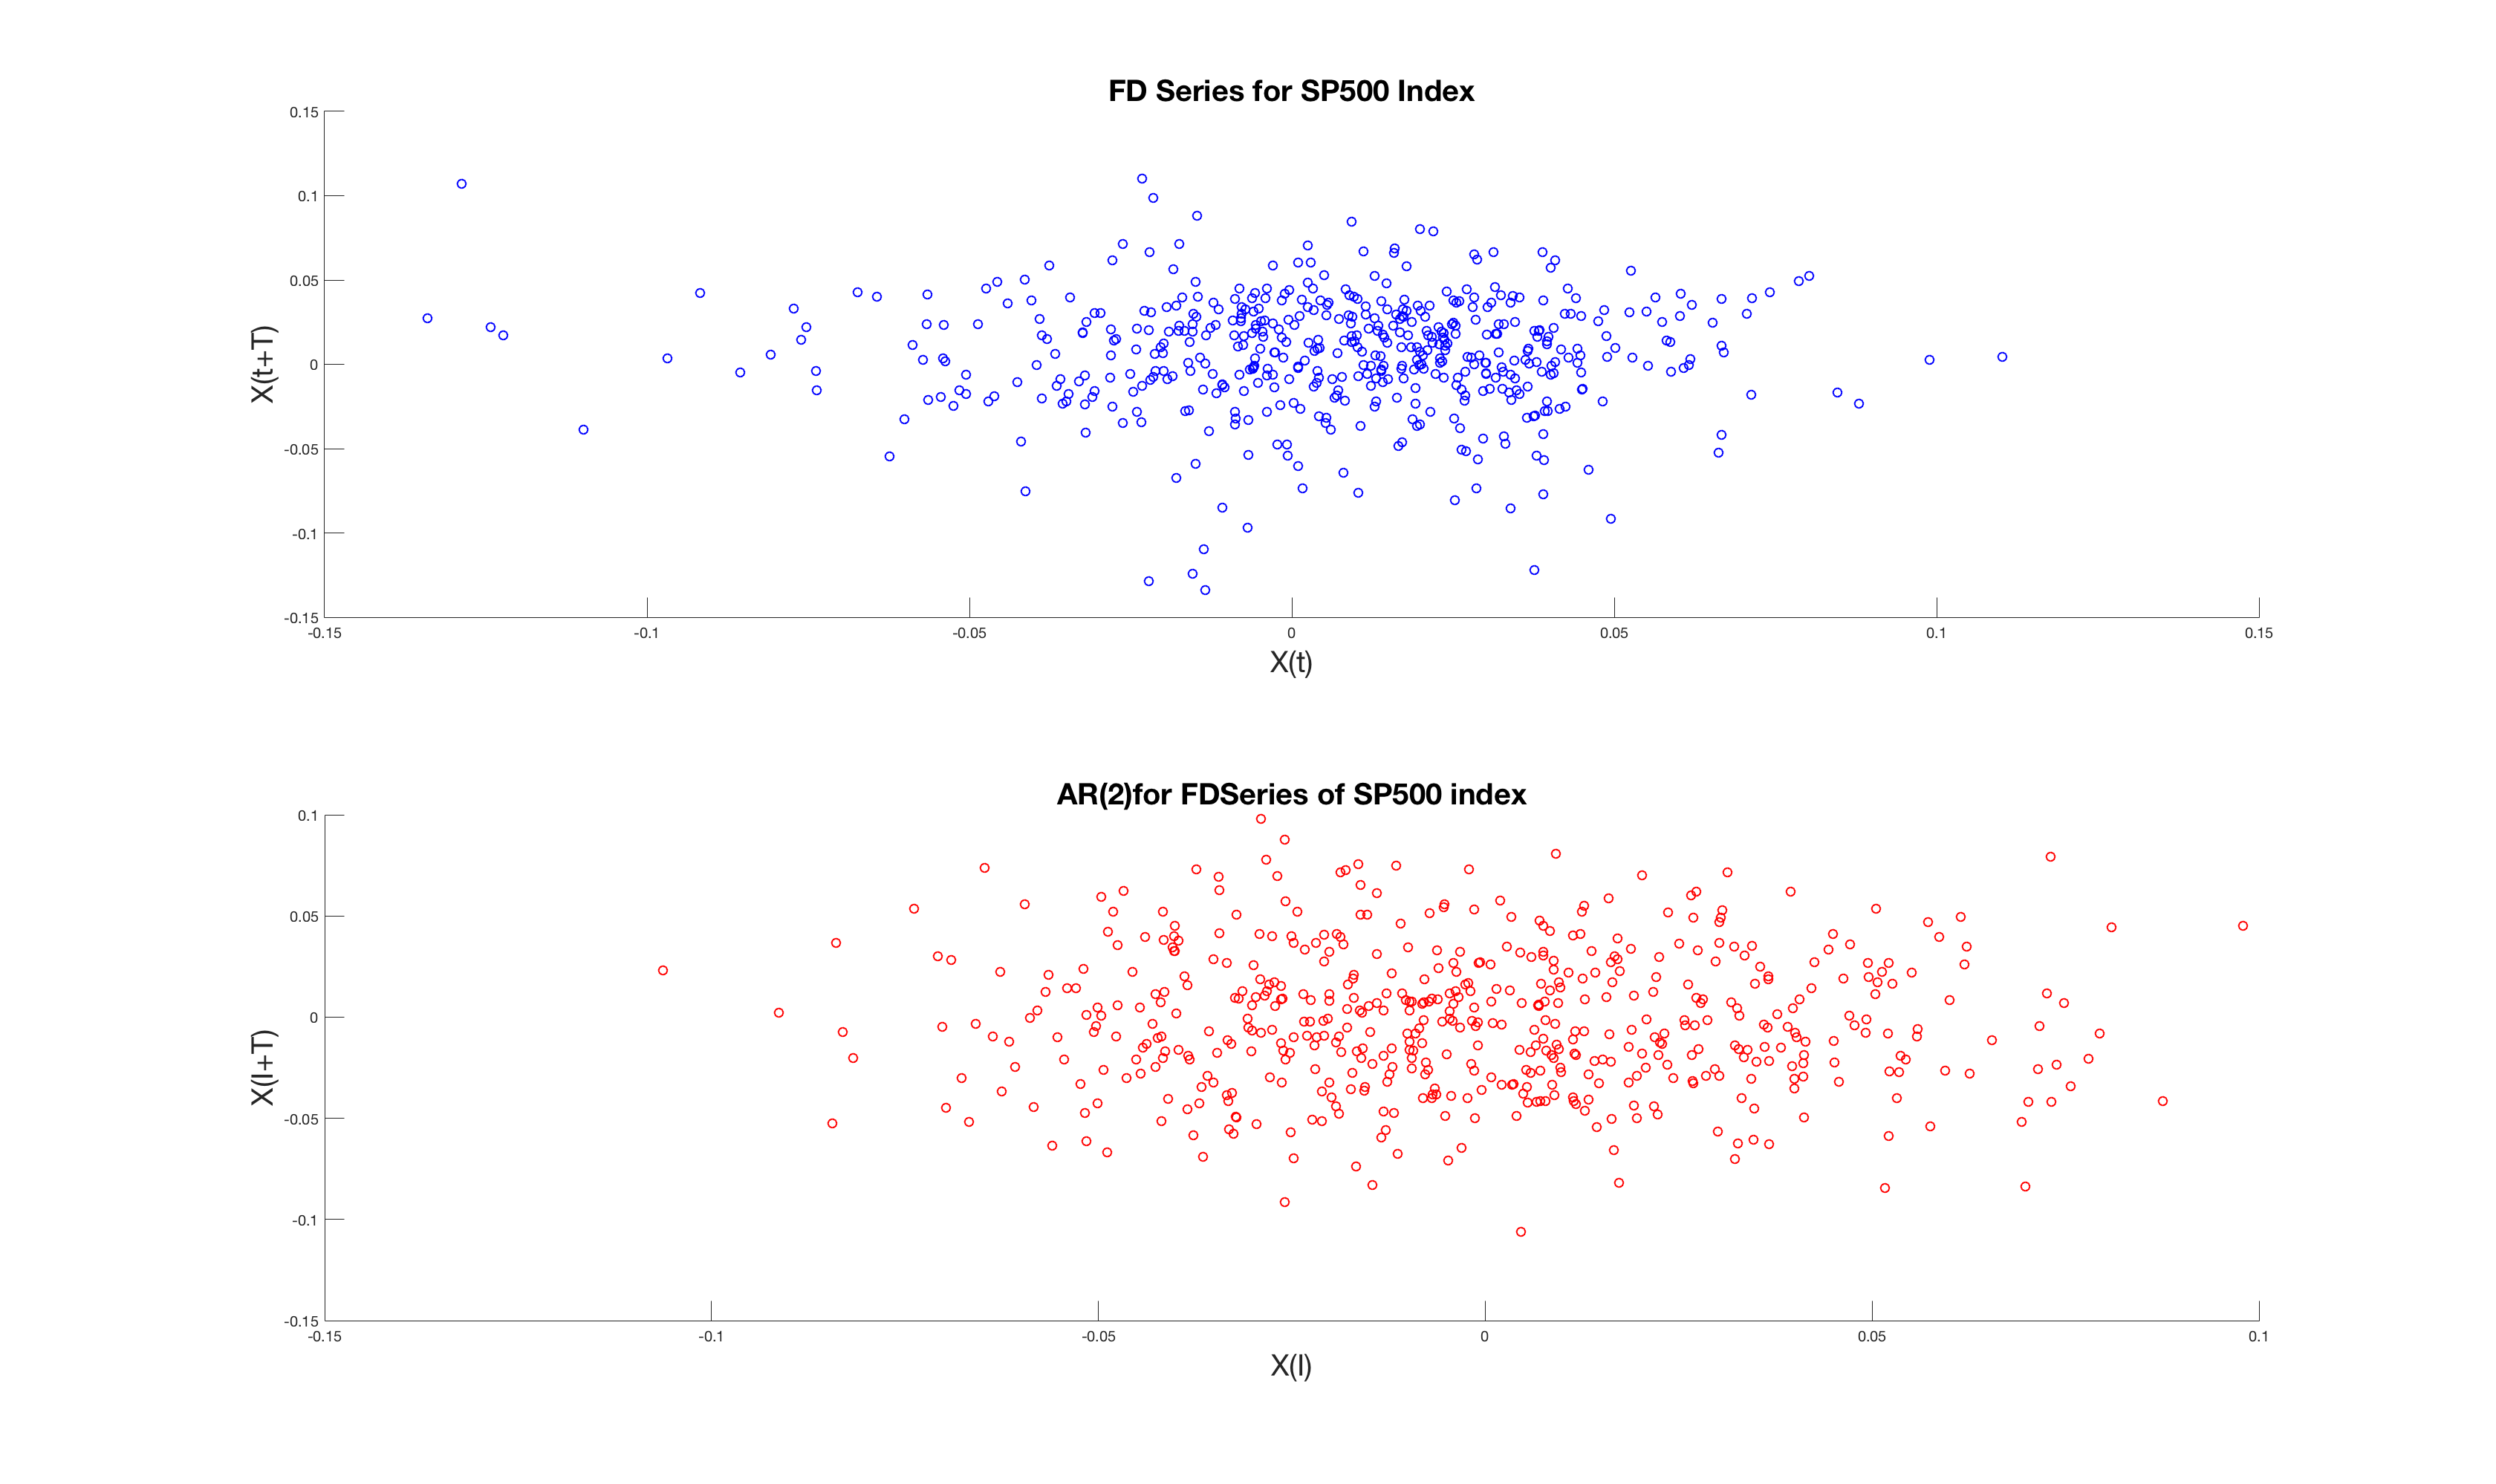
\includegraphics[scale=.15]{Images/FDAR2SP500}
\caption{Fig a) SP500 FD Series. T = 40. The pattern demonstrates the existence of dominant of high frequency noise. Fig b) AR(2) for the FD Series of SP500. T=5. The program used to create the graph is myFDFilter.m and it is attached in the appendix B.}
\label{fig:FDAR2SP500}
\end{figure}


\begin{figure}[!ht]
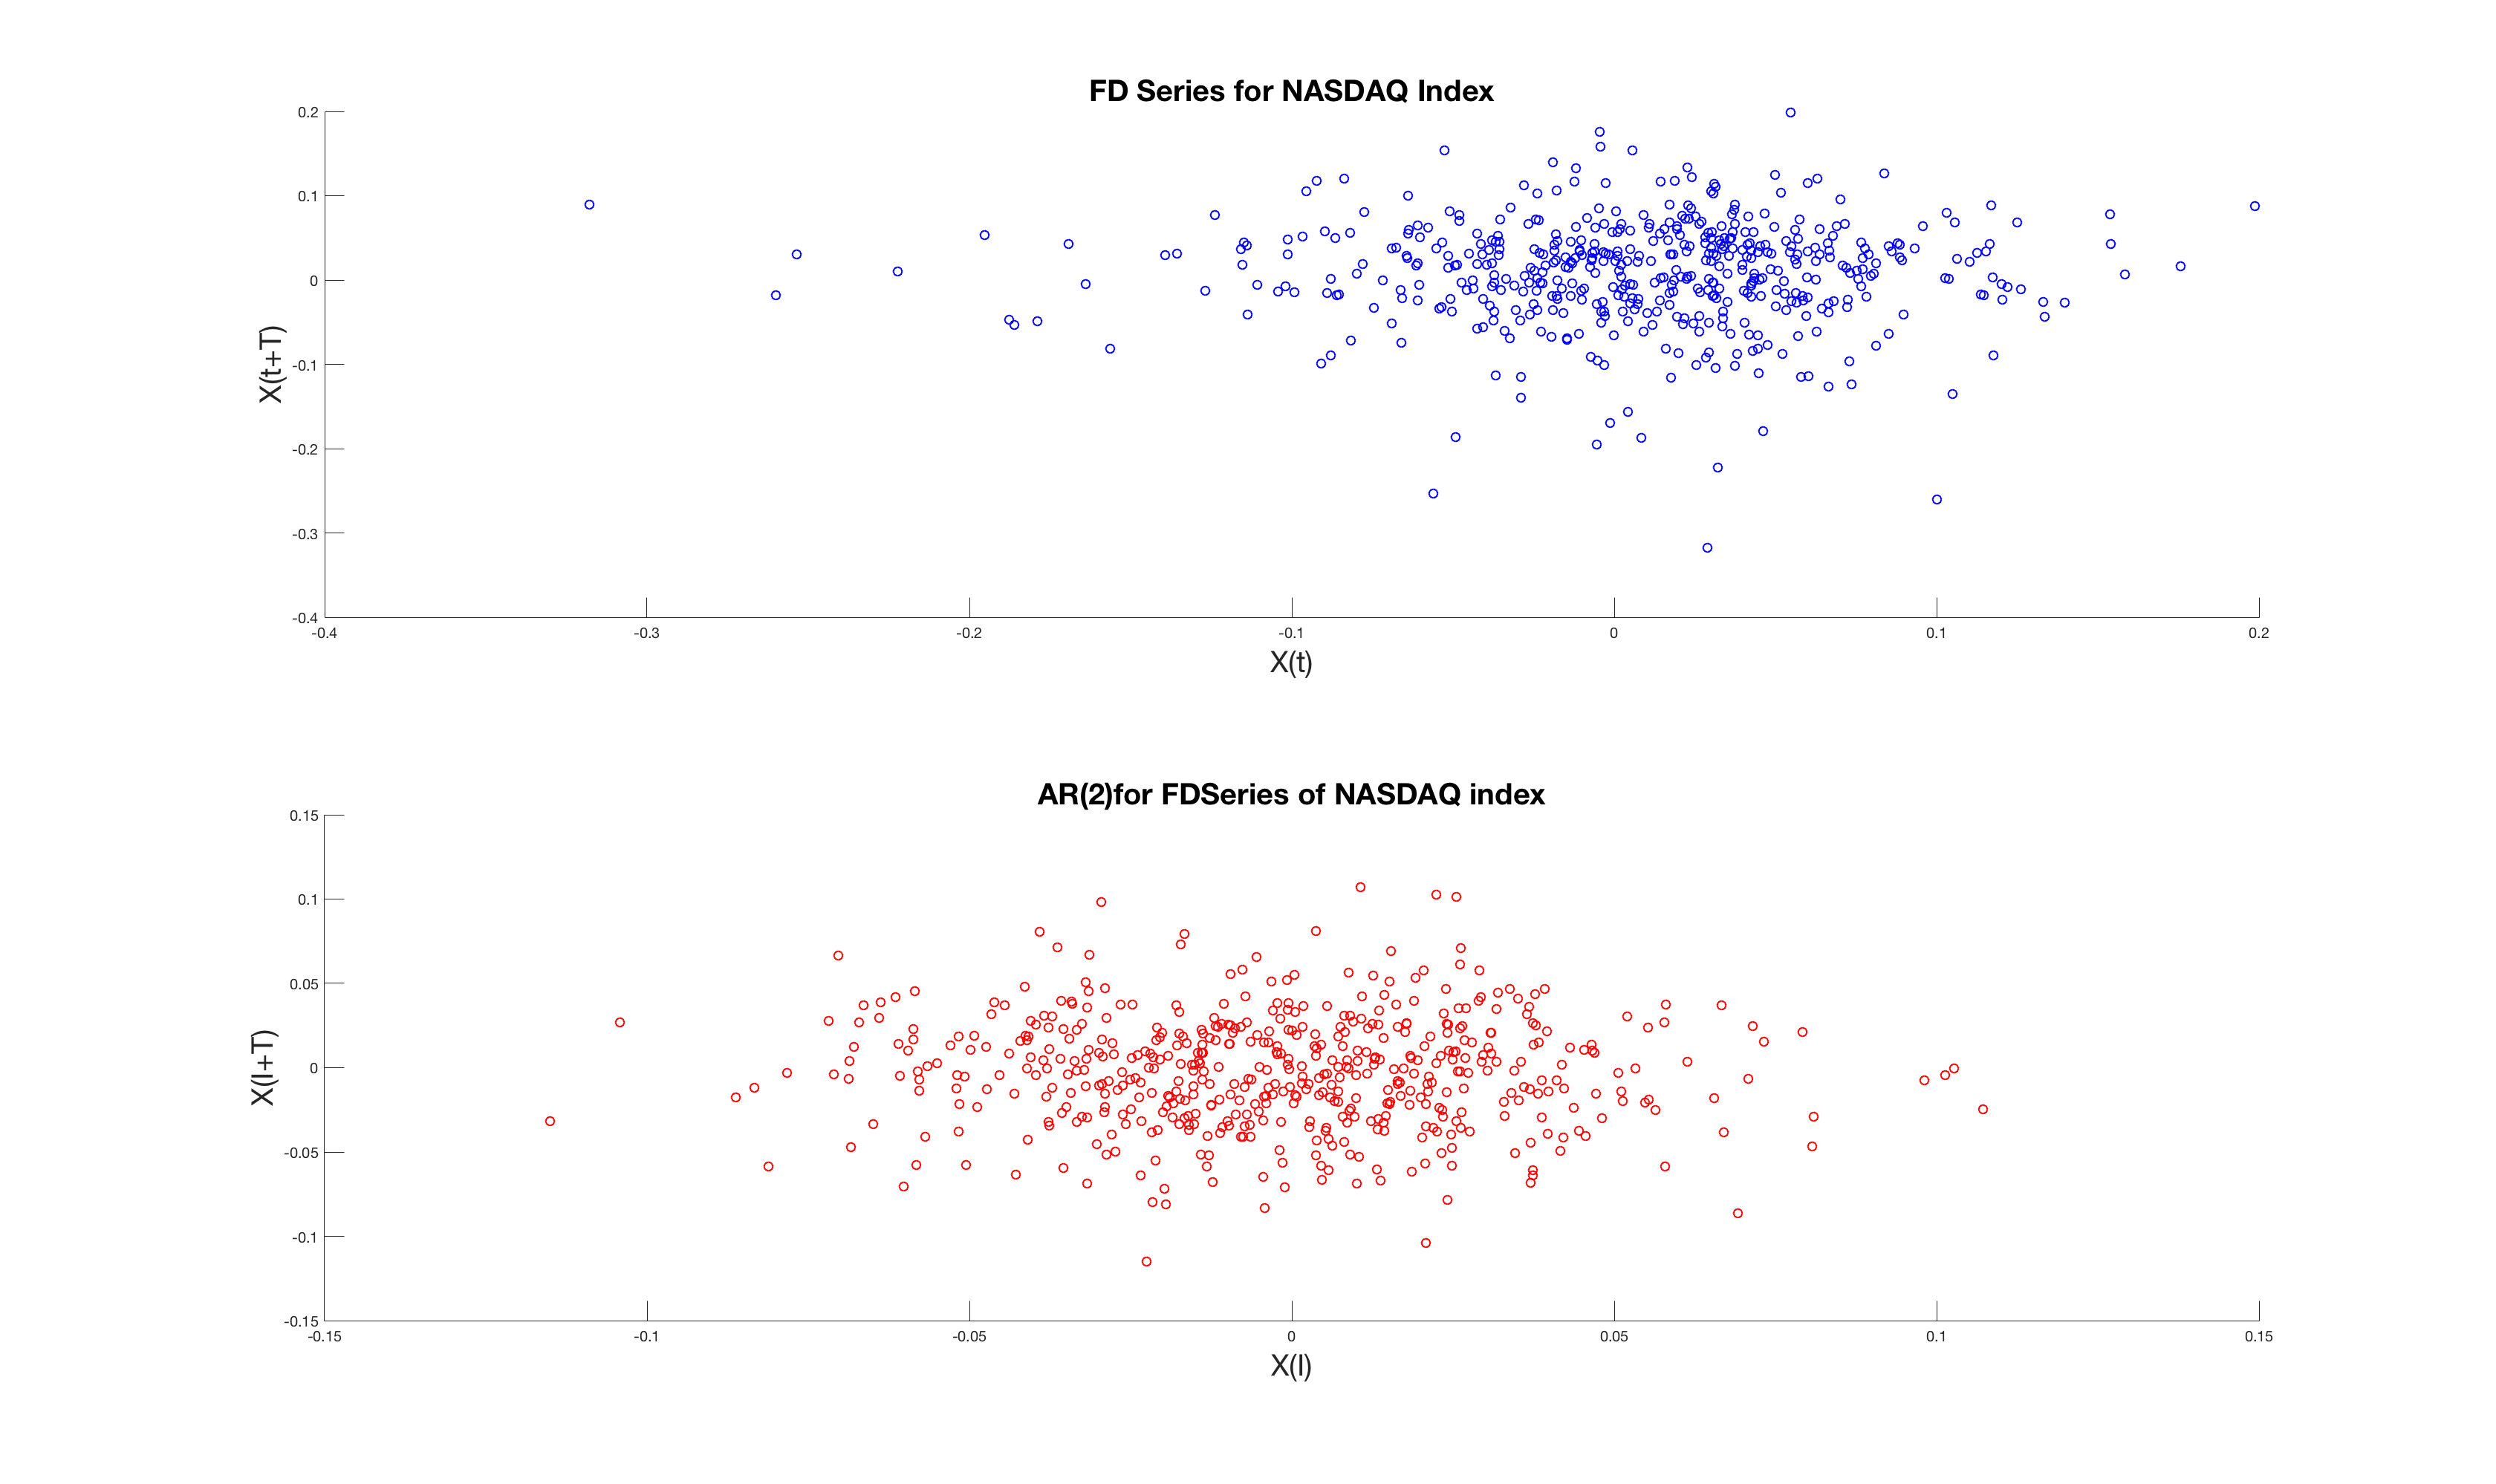
\includegraphics[scale=.15]{Images/FDAR2NASDAQ}
\caption{Fig a) NASDAQ FD Series. T = 40. The pattern demonstrates the existence of dominant of high frequency noise. Fig b) AR(2) for the FD Series of NASDAQ. T=5. The program used to create the graph is myFDFilter.m and it is attached in the appendix B.}
\label{fig:FDAR2NASDAQ}
\end{figure}

\begin{table}[h!]
\centering
\begin{tabular}{||c c c c c c c c c||}
 \hline
  Data & $\eta$ & $\nu(\%)$ & CCgo & $P_{c}$  & $\phi (\%)$ & $P_{dc}$ & $\lambda^{-1}$ &$\mu$ \\ [0.5ex]
   \hline\hline
    SP500 & 1.032 & 106.6 & 0.4141 & NA & NA & NA & NA\\
	 NASDAQ & 1.0116 & 102.33 & 0.4735 & NA & NA & NA & NA \\
	   \hline
	   \end{tabular}
	   \caption{Detrend Statistics on S\&P 500 }
	   \label{table:dectrendstat}
	   \end{table}
\subsection{Conclusion}
Color chaos model uncovers the business cycle in the stock market indices SP500 and NASDAQ and existence of persistent cycles reveals a new perspective of market. The study provides additional clarity on the opportunity in studying stock market movements using the joint time frequency analysis. A new study was performed by rearranging the indices value randomly instead of being time dependent, similar color chaos models was applied. The initial results of this new study revealed a similar cycles in the stock market. The results of this new study is not attached to this report but provides an opportunity to continue the study market behavior by converting the market indices value time independent. Further study may reveal more deeper understanding of the market behavior.

